% Digital Logic Report Template
% Created: 2020-01-10, John Miller

%==========================================================
%=========== Document Setup  ==============================

% Formatting defined by class file
\documentclass[11pt]{article}

% ---- Document formatting ----
\usepackage[margin=1in]{geometry}	% Narrower margins
\usepackage{booktabs}				% Nice formatting of tables
\usepackage{graphicx}				% Ability to include graphics

%\setlength\parindent{0pt}	% Do not indent first line of paragraphs 
\usepackage[parfill]{parskip}		% Line space b/w paragraphs
%	parfill option prevents last line of pgrph from being fully justified

% Parskip package adds too much space around titles, fix with this
\RequirePackage{titlesec}
\titlespacing\section{0pt}{8pt plus 4pt minus 2pt}{3pt plus 2pt minus 2pt}
\titlespacing\subsection{0pt}{4pt plus 4pt minus 2pt}{-2pt plus 2pt minus 2pt}
\titlespacing\subsubsection{0pt}{2pt plus 4pt minus 2pt}{-6pt plus 2pt minus 2pt}

% ---- Hyperlinks ----
\usepackage[colorlinks=true,urlcolor=blue]{hyperref}	% For URL's. Automatically links internal references.

% ---- Code listings ----
\usepackage{listings} 					% Nice code layout and inclusion
\usepackage[usenames,dvipsnames]{xcolor}	% Colors (needs to be defined before using colors)

% Define custom colors for listings
\definecolor{listinggray}{gray}{0.98}		% Listings background color
\definecolor{rulegray}{gray}{0.7}			% Listings rule/frame color

% Style for Verilog
\lstdefinestyle{Verilog}{
	language=Verilog,					% Verilog
	backgroundcolor=\color{listinggray},	% light gray background
	rulecolor=\color{blue}, 			% blue frame lines
	frame=tb,							% lines above & below
	linewidth=\columnwidth, 			% set line width
	basicstyle=\small\ttfamily,	% basic font style that is used for the code	
	breaklines=true, 					% allow breaking across columns/pages
	tabsize=3,							% set tab size
	commentstyle=\color{gray},	% comments in italic 
	stringstyle=\upshape,				% strings are printed in normal font
	showspaces=false,					% don't underscore spaces
}

% How to use: \Verilog[listing_options]{file}
\newcommand{\Verilog}[2][]{%
	\lstinputlisting[style=Verilog,#1]{#2}
}




%======================================================
%=========== Body  ====================================
\begin{document}

\title{ELC 2137 Lab 08: 4-Digit Display}
\author{Abigail Joseph}

\maketitle


\section*{Summary}

In this lab, we used modules from previous labs to create a 4-digit display that can output either hexadecimal or BCD values. We created some larger muxes and an anode decoder.   

\section*{Code}

\Verilog[firstline=23, caption=Mux 2 ,label=code:file_1]{mux2.sv}
\Verilog[firstline=23, caption=Mux 2 Testbench ,label=code:file_2]{mux2_test.sv}
\Verilog[firstline=23, caption=Mux 4 ,label=code:file_3]{mux4.sv}
\Verilog[firstline=23, caption=Mux 4 Testbench ,label=code:file_4]{mux4_test.sv}
\Verilog[firstline=23, caption=Anode Decoder ,label=code:file_5]{an_decoder.sv}
\Verilog[firstline=23, caption=Anode Decoder Testbench ,label=code:file_6]{an_decoder_test.sv}
\Verilog[firstline=23, caption=Seven Segment 4 ,label=code:file_7]{sseg4.sv}
\Verilog[firstline=23, caption=Manual ,label=code:file_8]{sseg4_manual.sv}

\section*{Results}

\begin{figure}[ht] \centering
	
	\begin{tabular}{c|c}
		\toprule
		in & out \\
		\midrule
		00 & 1110 \\
		01 & 1101 \\
		10 & 1011 \\
		11 & 0111 \\
		\bottomrule
	\end{tabular}
	
	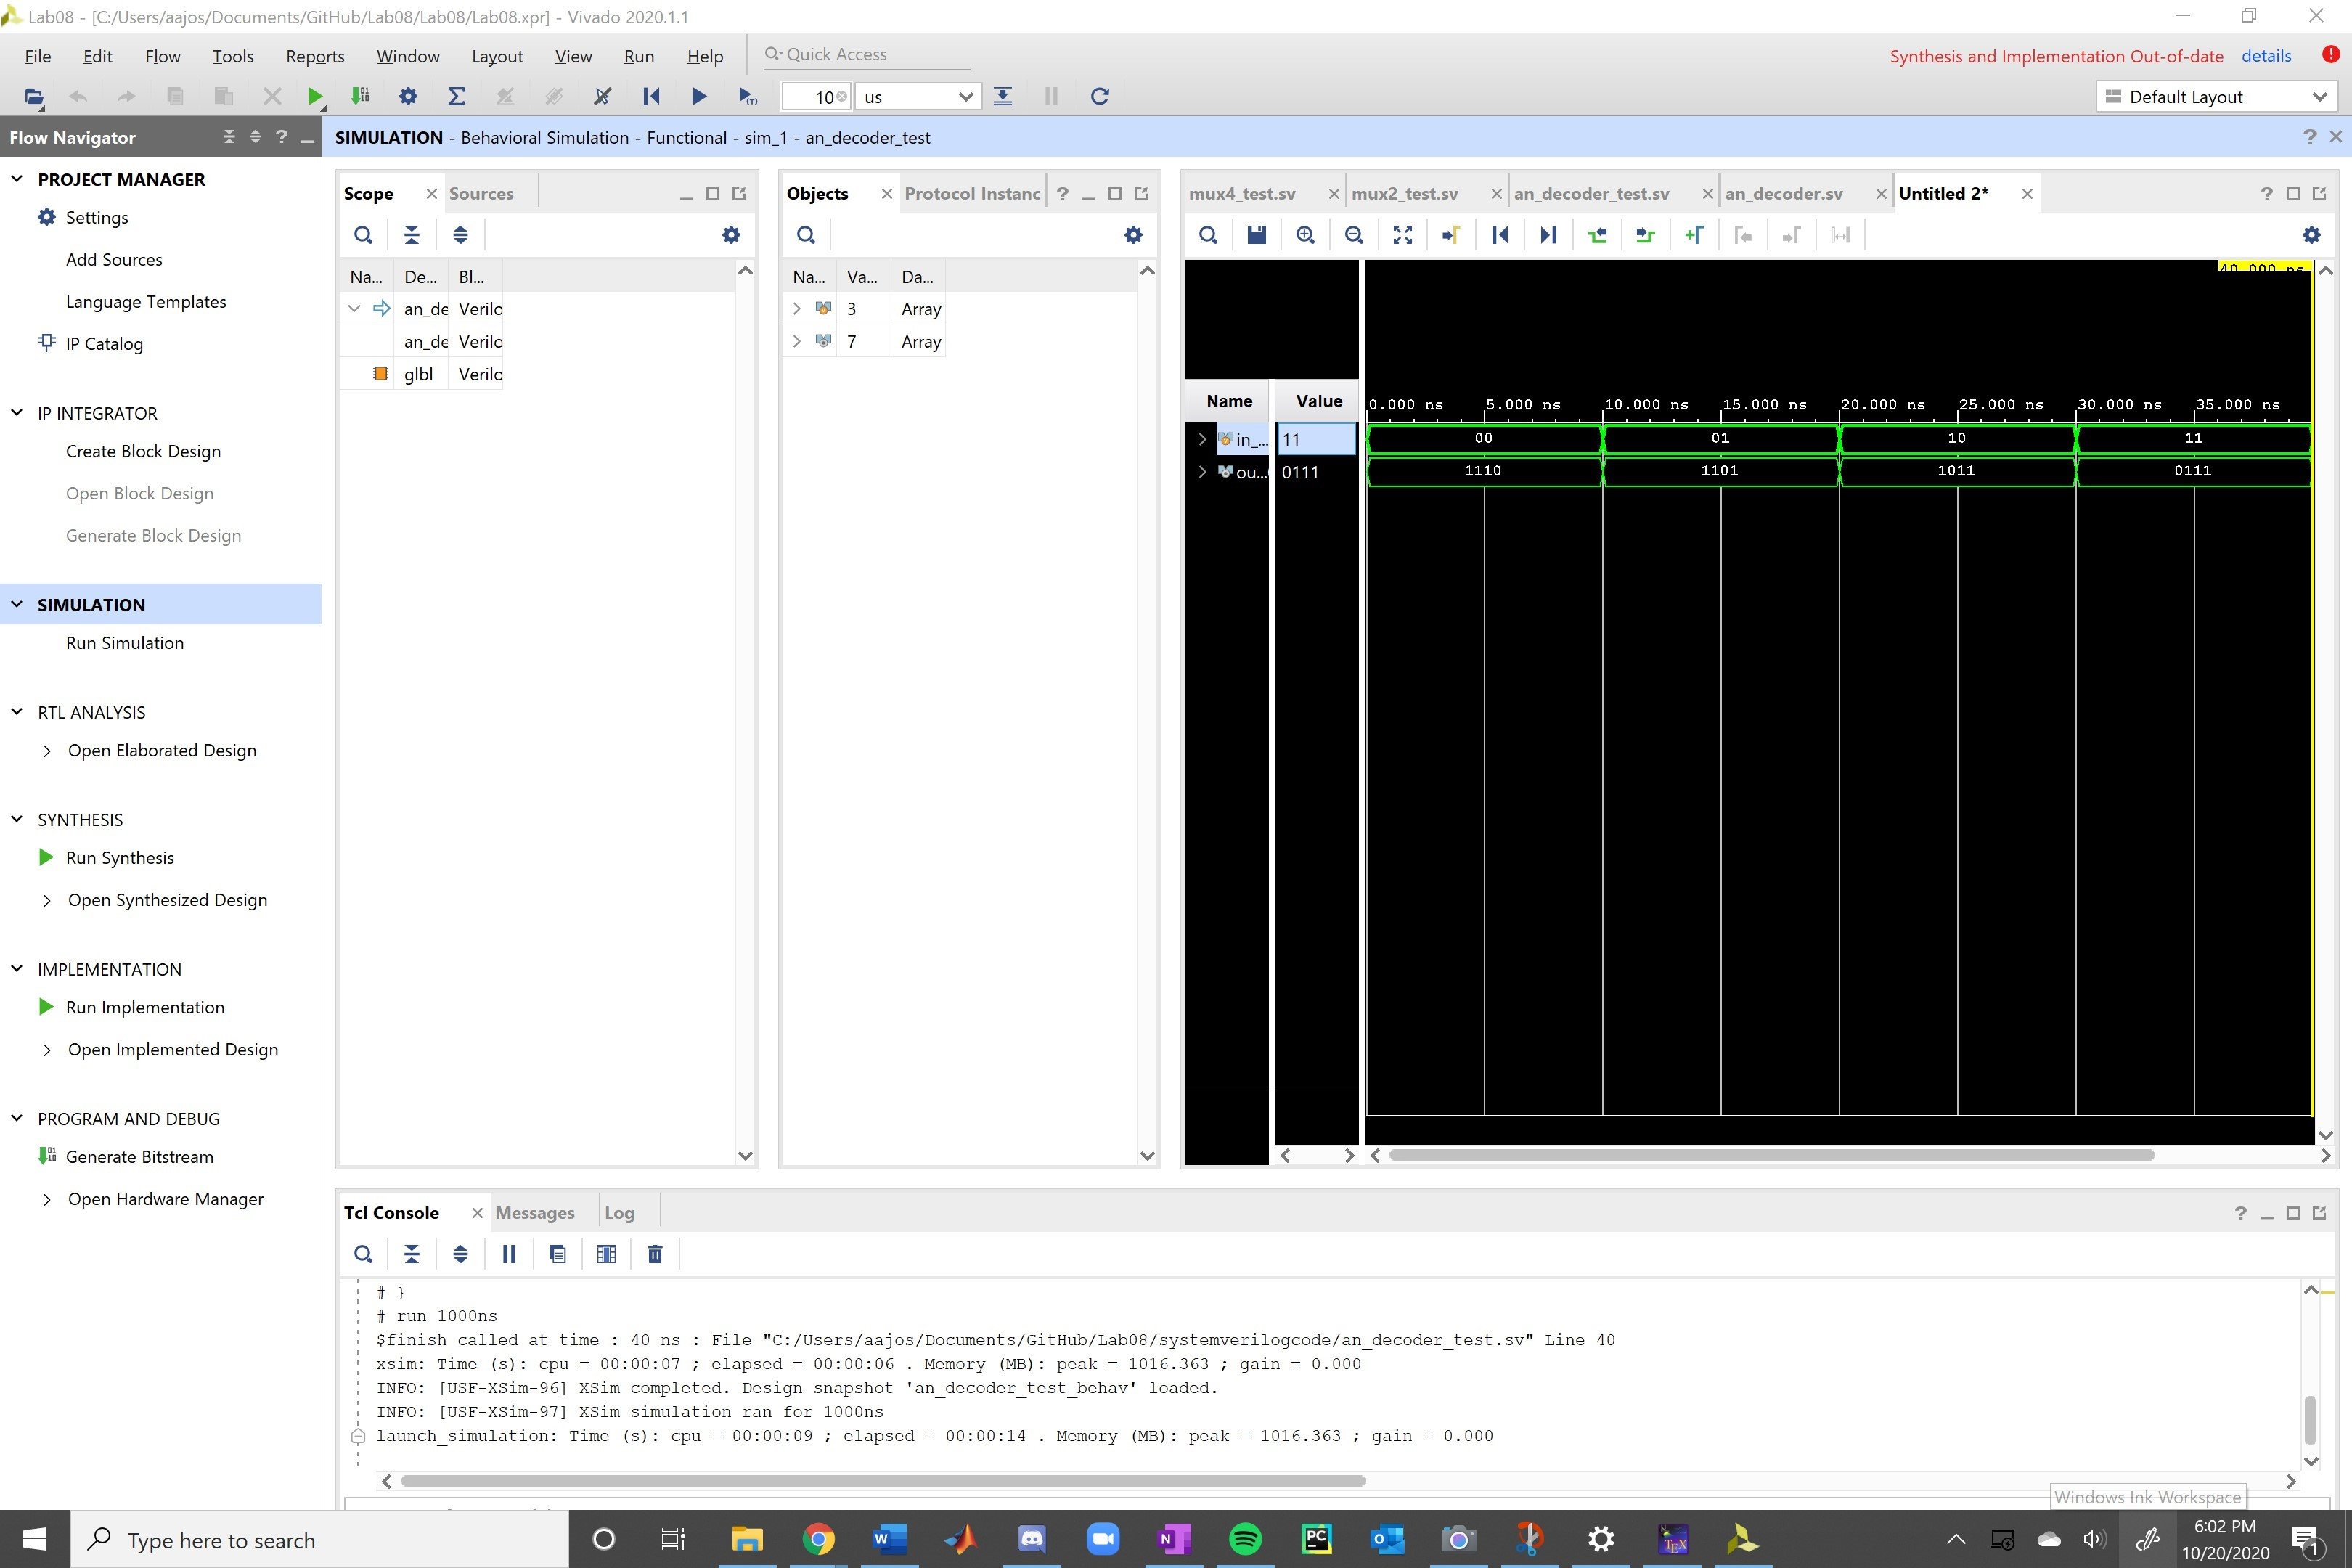
\includegraphics[width=1\textwidth,trim=19cm 19cm 0cm 6cm,clip]{an_decoder_test_scrn}
	\caption{Anode Decoder Simulation}
	\label{fig:img3}
\end{figure}

\begin{figure}[ht] \centering
	
	\begin{tabular}{ccc|c}
		\toprule
		in0 & in1 & sel & out \\
		\midrule
		0 & 0010 & 1001 & 0010 \\
		1 & 0010 & 1001 & 1001 \\
		0 & 0001 & 0100 & 0001 \\
		1 & 0001 & 0100 & 0100 \\
		\bottomrule
	\end{tabular}
	
	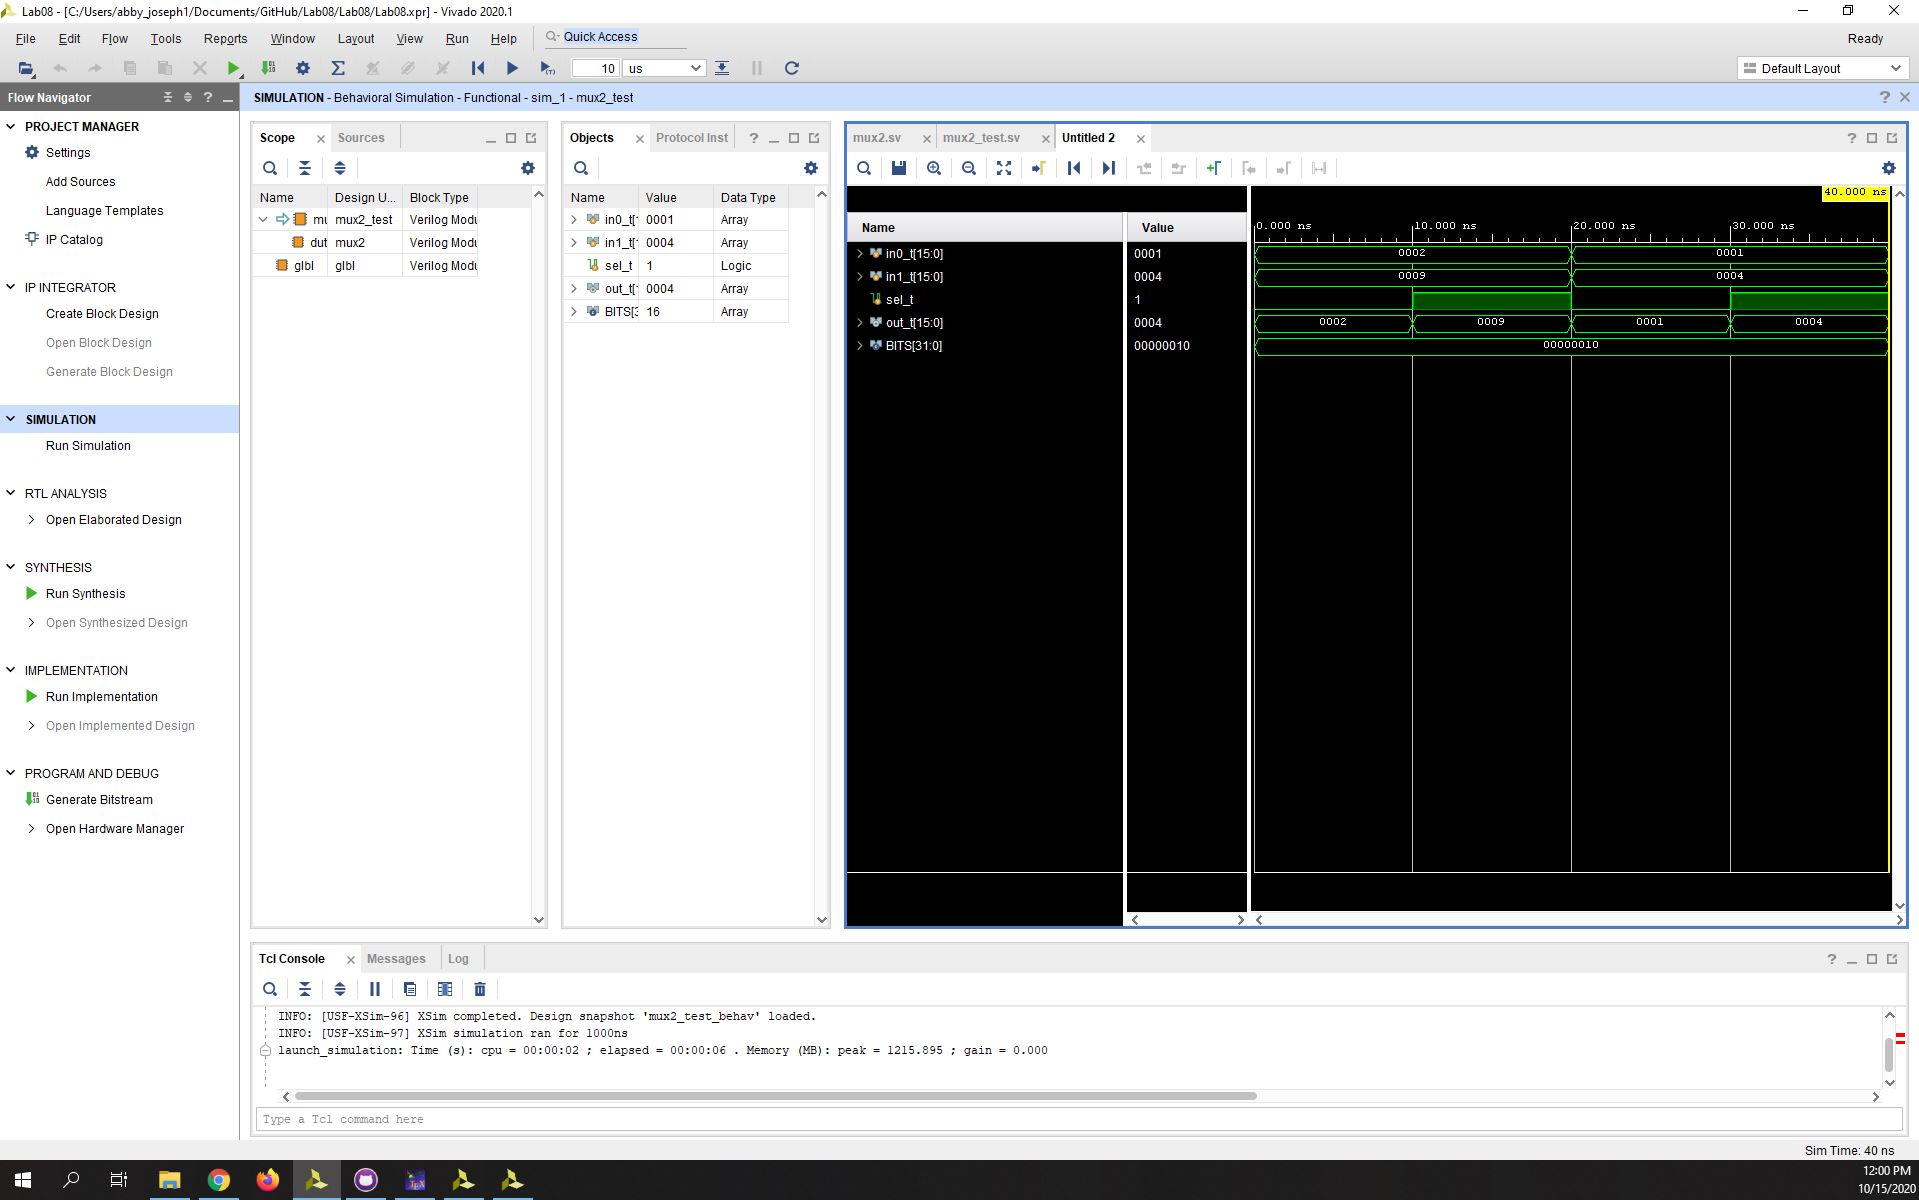
\includegraphics[width=1\textwidth,trim=21cm 19cm 0cm 6cm,clip]{mux2_test_scrn}
	\caption{Mux 2 Simulation}
	\label{fig:img1}
\end{figure}

\begin{figure}[ht] \centering
	
	\begin{tabular}{ccccc|c}
		\toprule
		in0 & in1 & in2 & in3 & sel & out \\
		\midrule
		00 & 0010 & 1001 & 1110 & 1011 & 0010 \\
		01 & 0010 & 1001 & 1110 & 1011 & 1001 \\
		00 & 0001 & 0100 & 1101 & 1010 & 0001 \\
		01 & 0001 & 0100 & 1101 & 1010 & 0100 \\
		10 & 0010 & 1001 & 1110 & 1011 & 1110 \\
		11 & 0010 & 1001 & 1110 & 1011 & 1011 \\
		10 & 0001 & 0100 & 1101 & 1010 & 1101 \\
		11 & 0001 & 0100 & 1101 & 1010 & 1010 \\
		\bottomrule
	\end{tabular}
	
	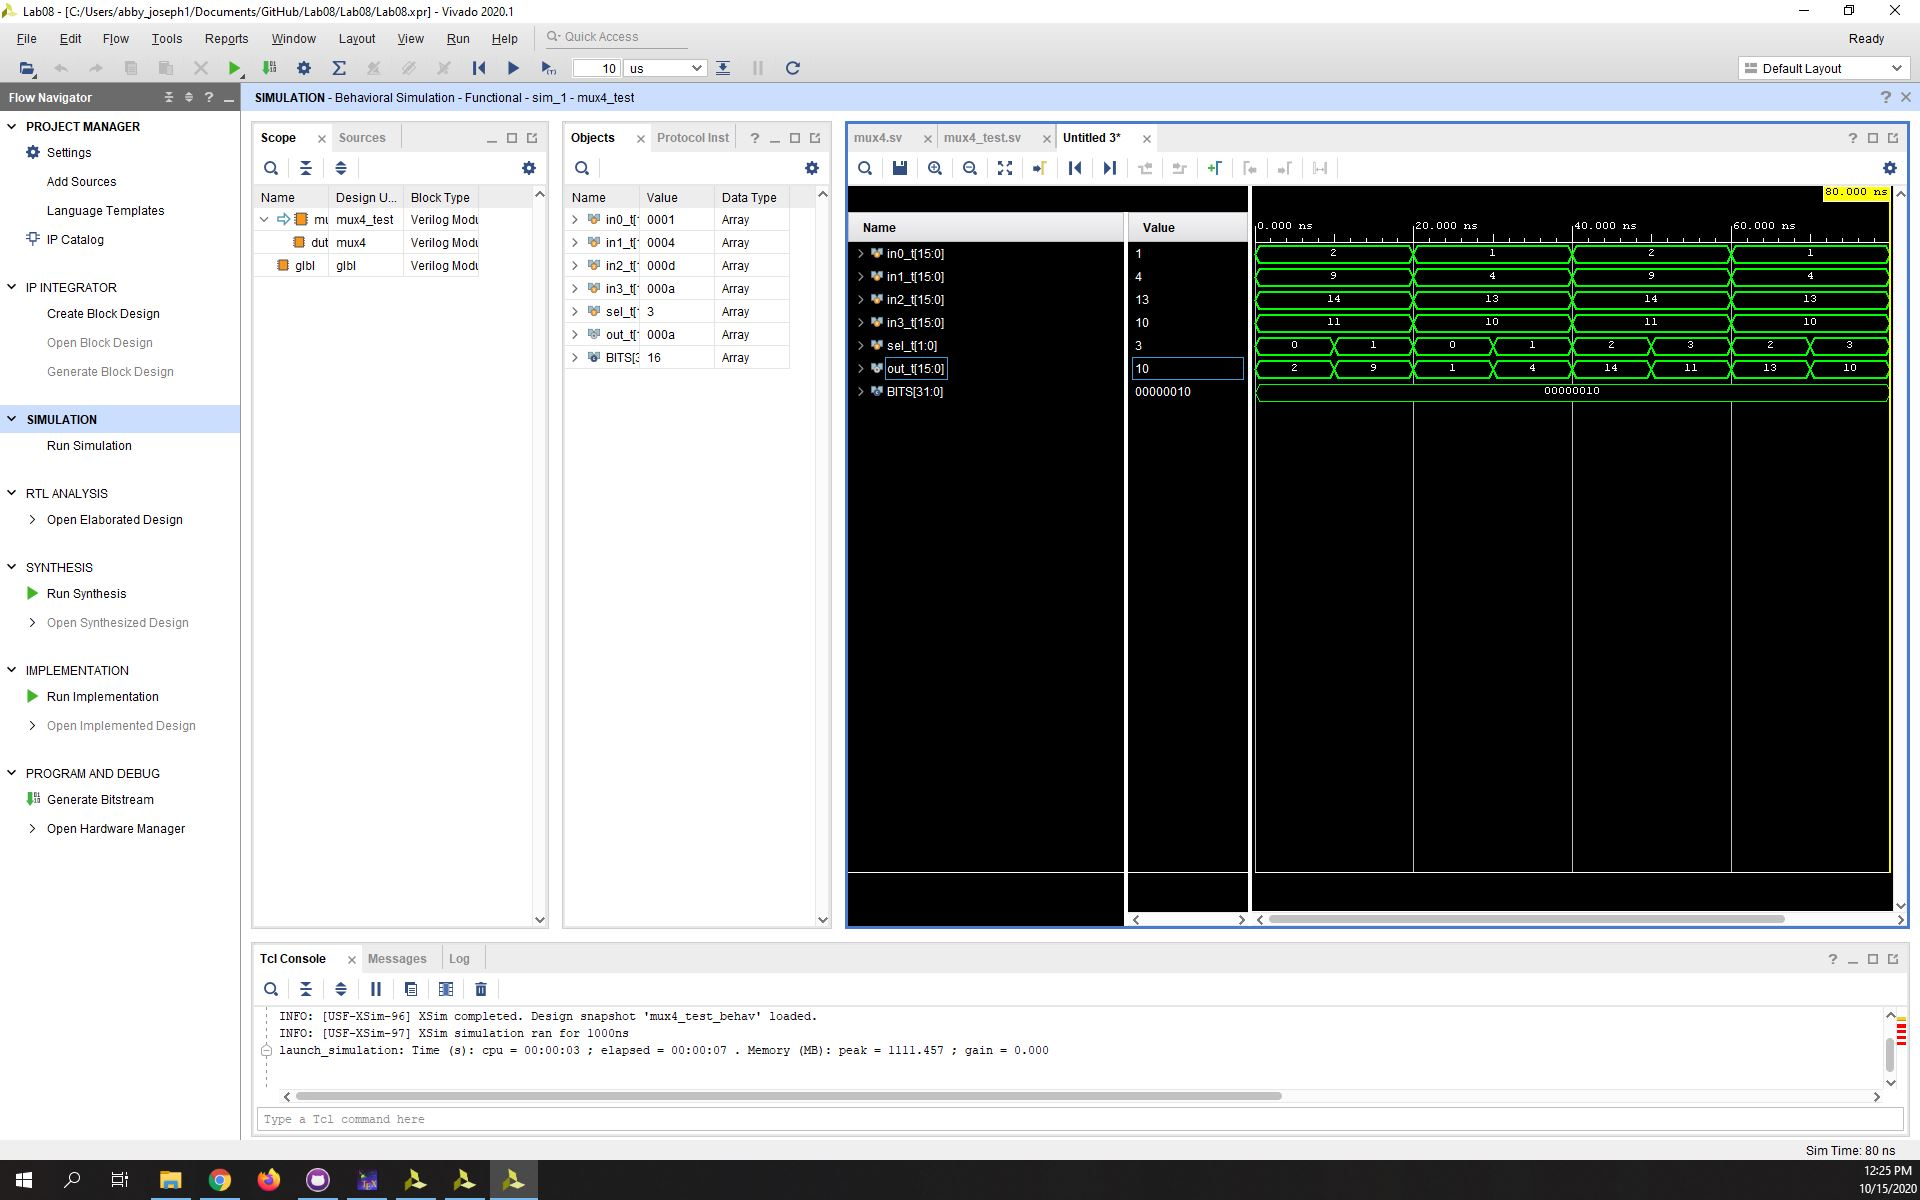
\includegraphics[width=1\textwidth,trim=21cm 19cm 0cm 6cm,clip]{mux4_test_scrn}
	\caption{Mux 4 Simulation}
	\label{fig:img2}
\end{figure}


\begin{figure}[ht]\centering
	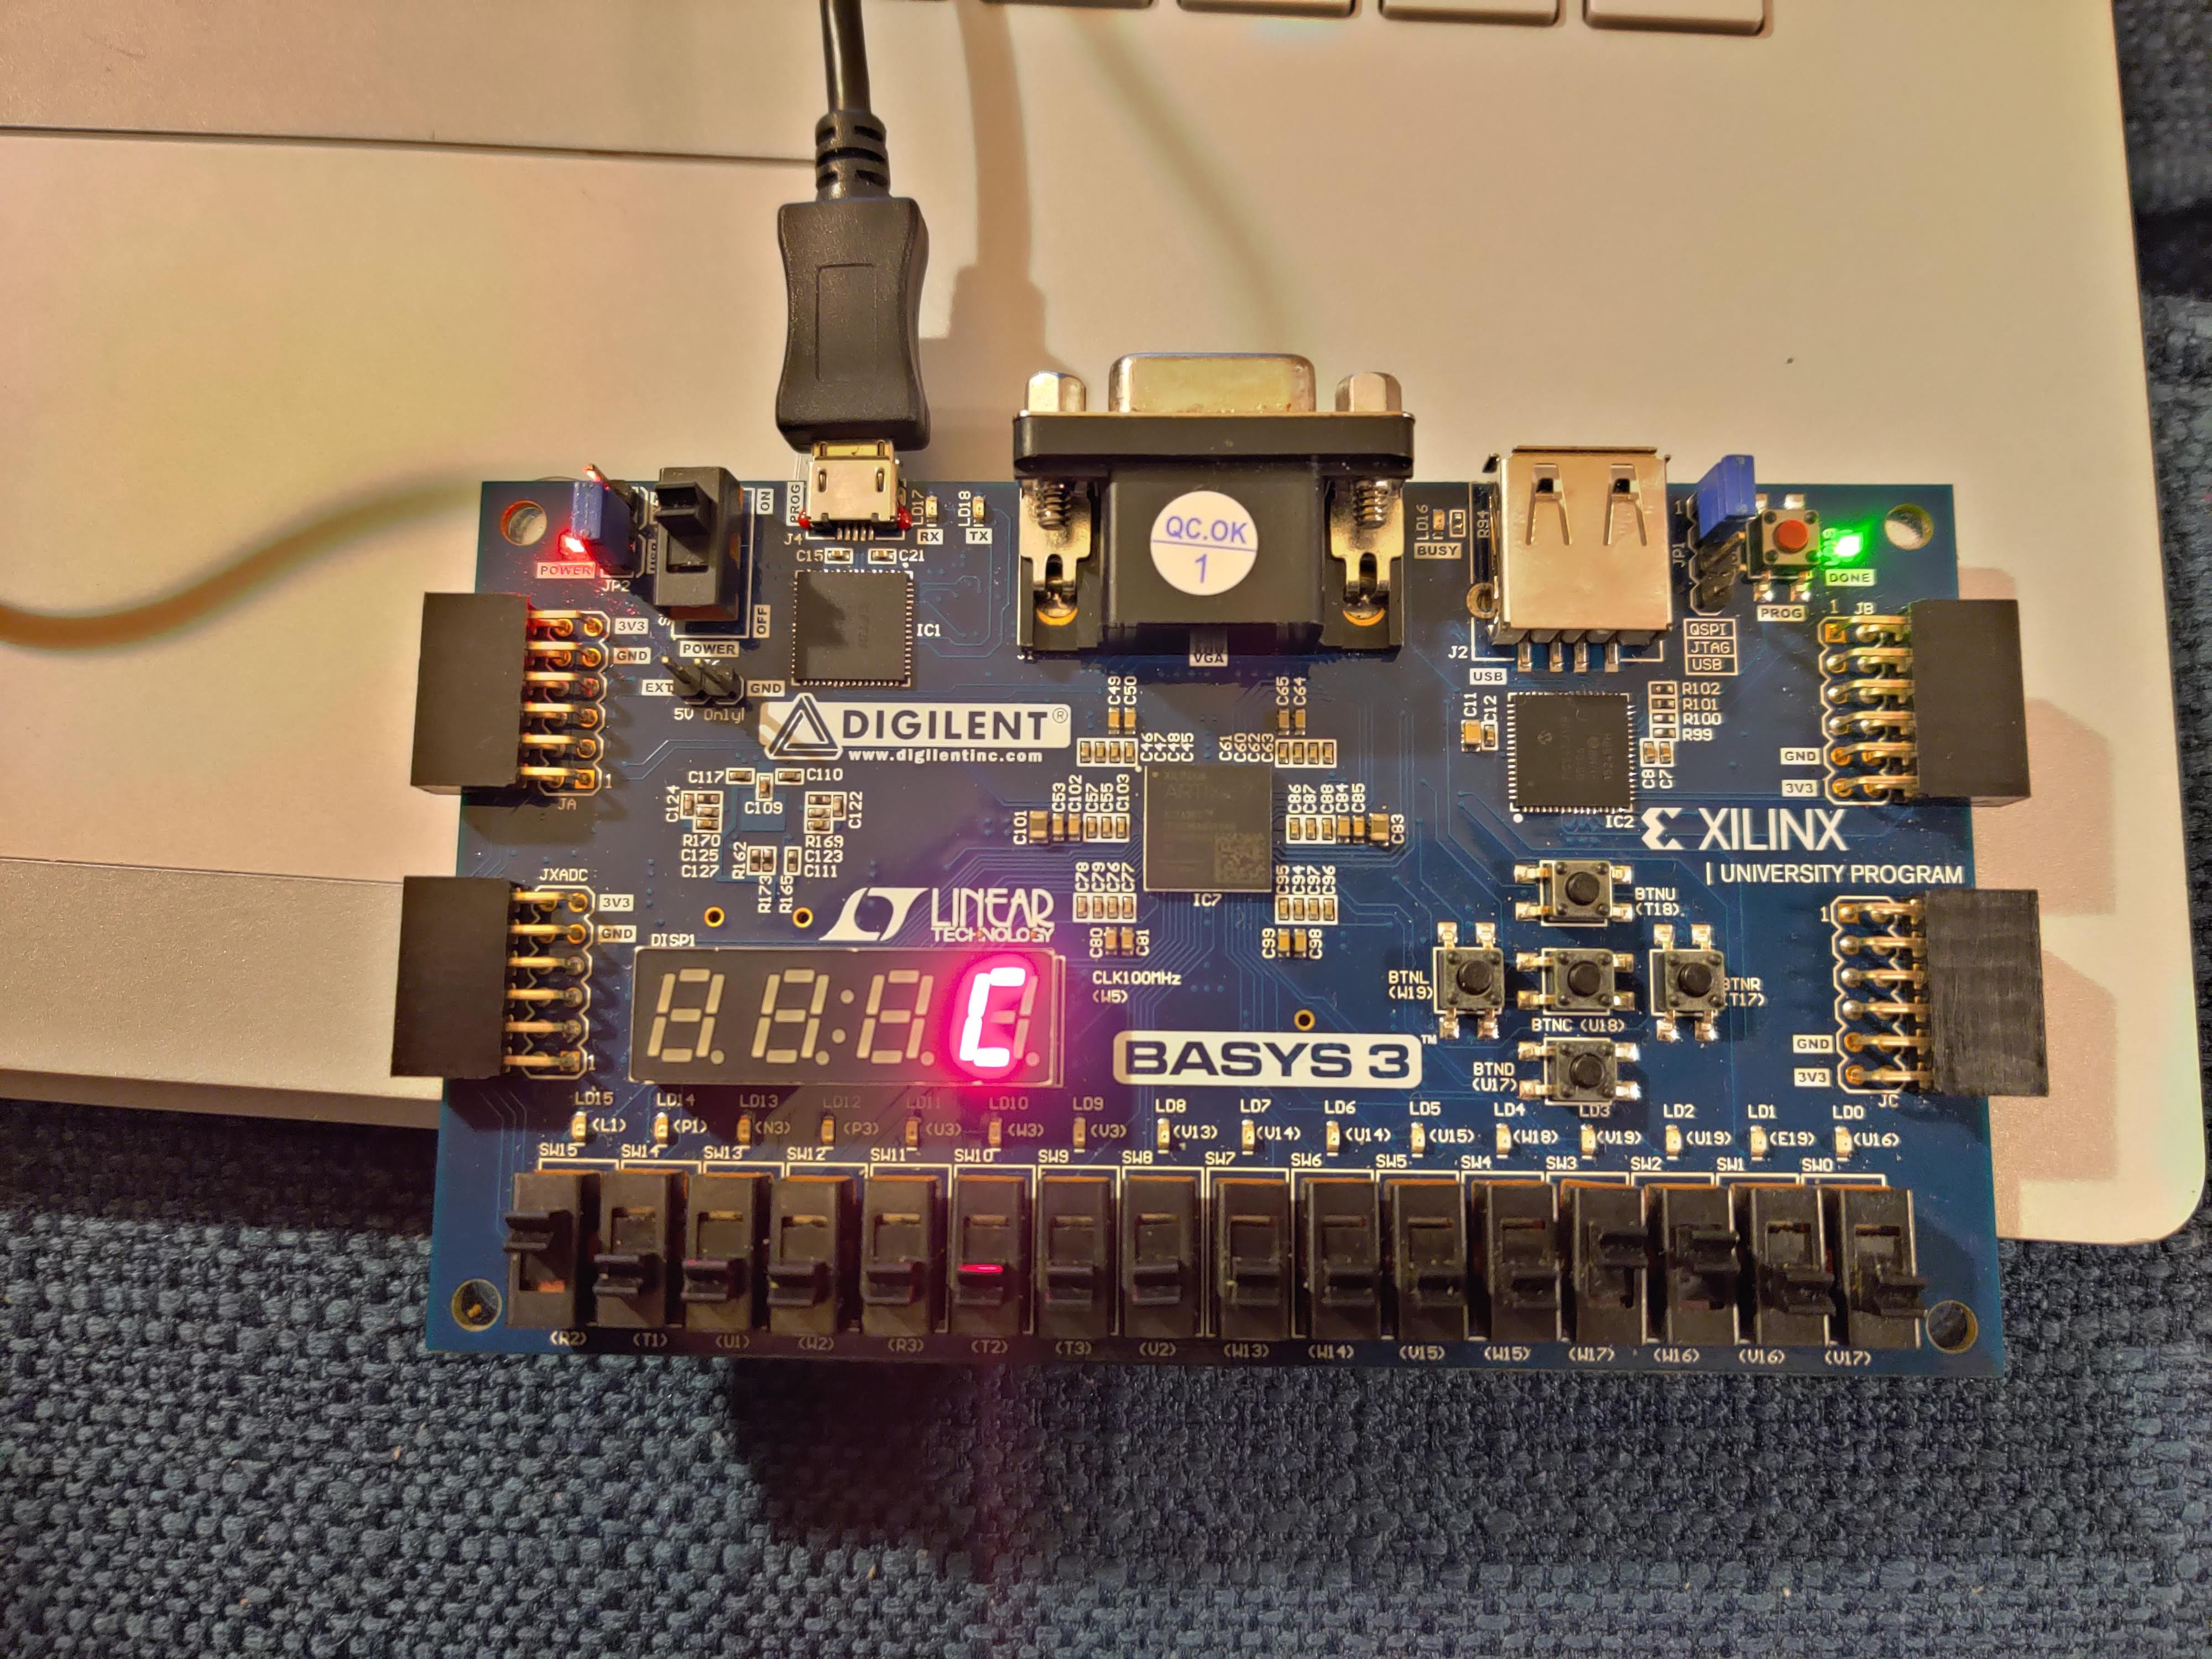
\includegraphics[width=.5\textwidth]{board1}
	\caption{1. sw15=1, sw3:0=1100, OUTPUT = C}
	\label{fig:b3_1}			
\end{figure}

\begin{figure}[ht]\centering
	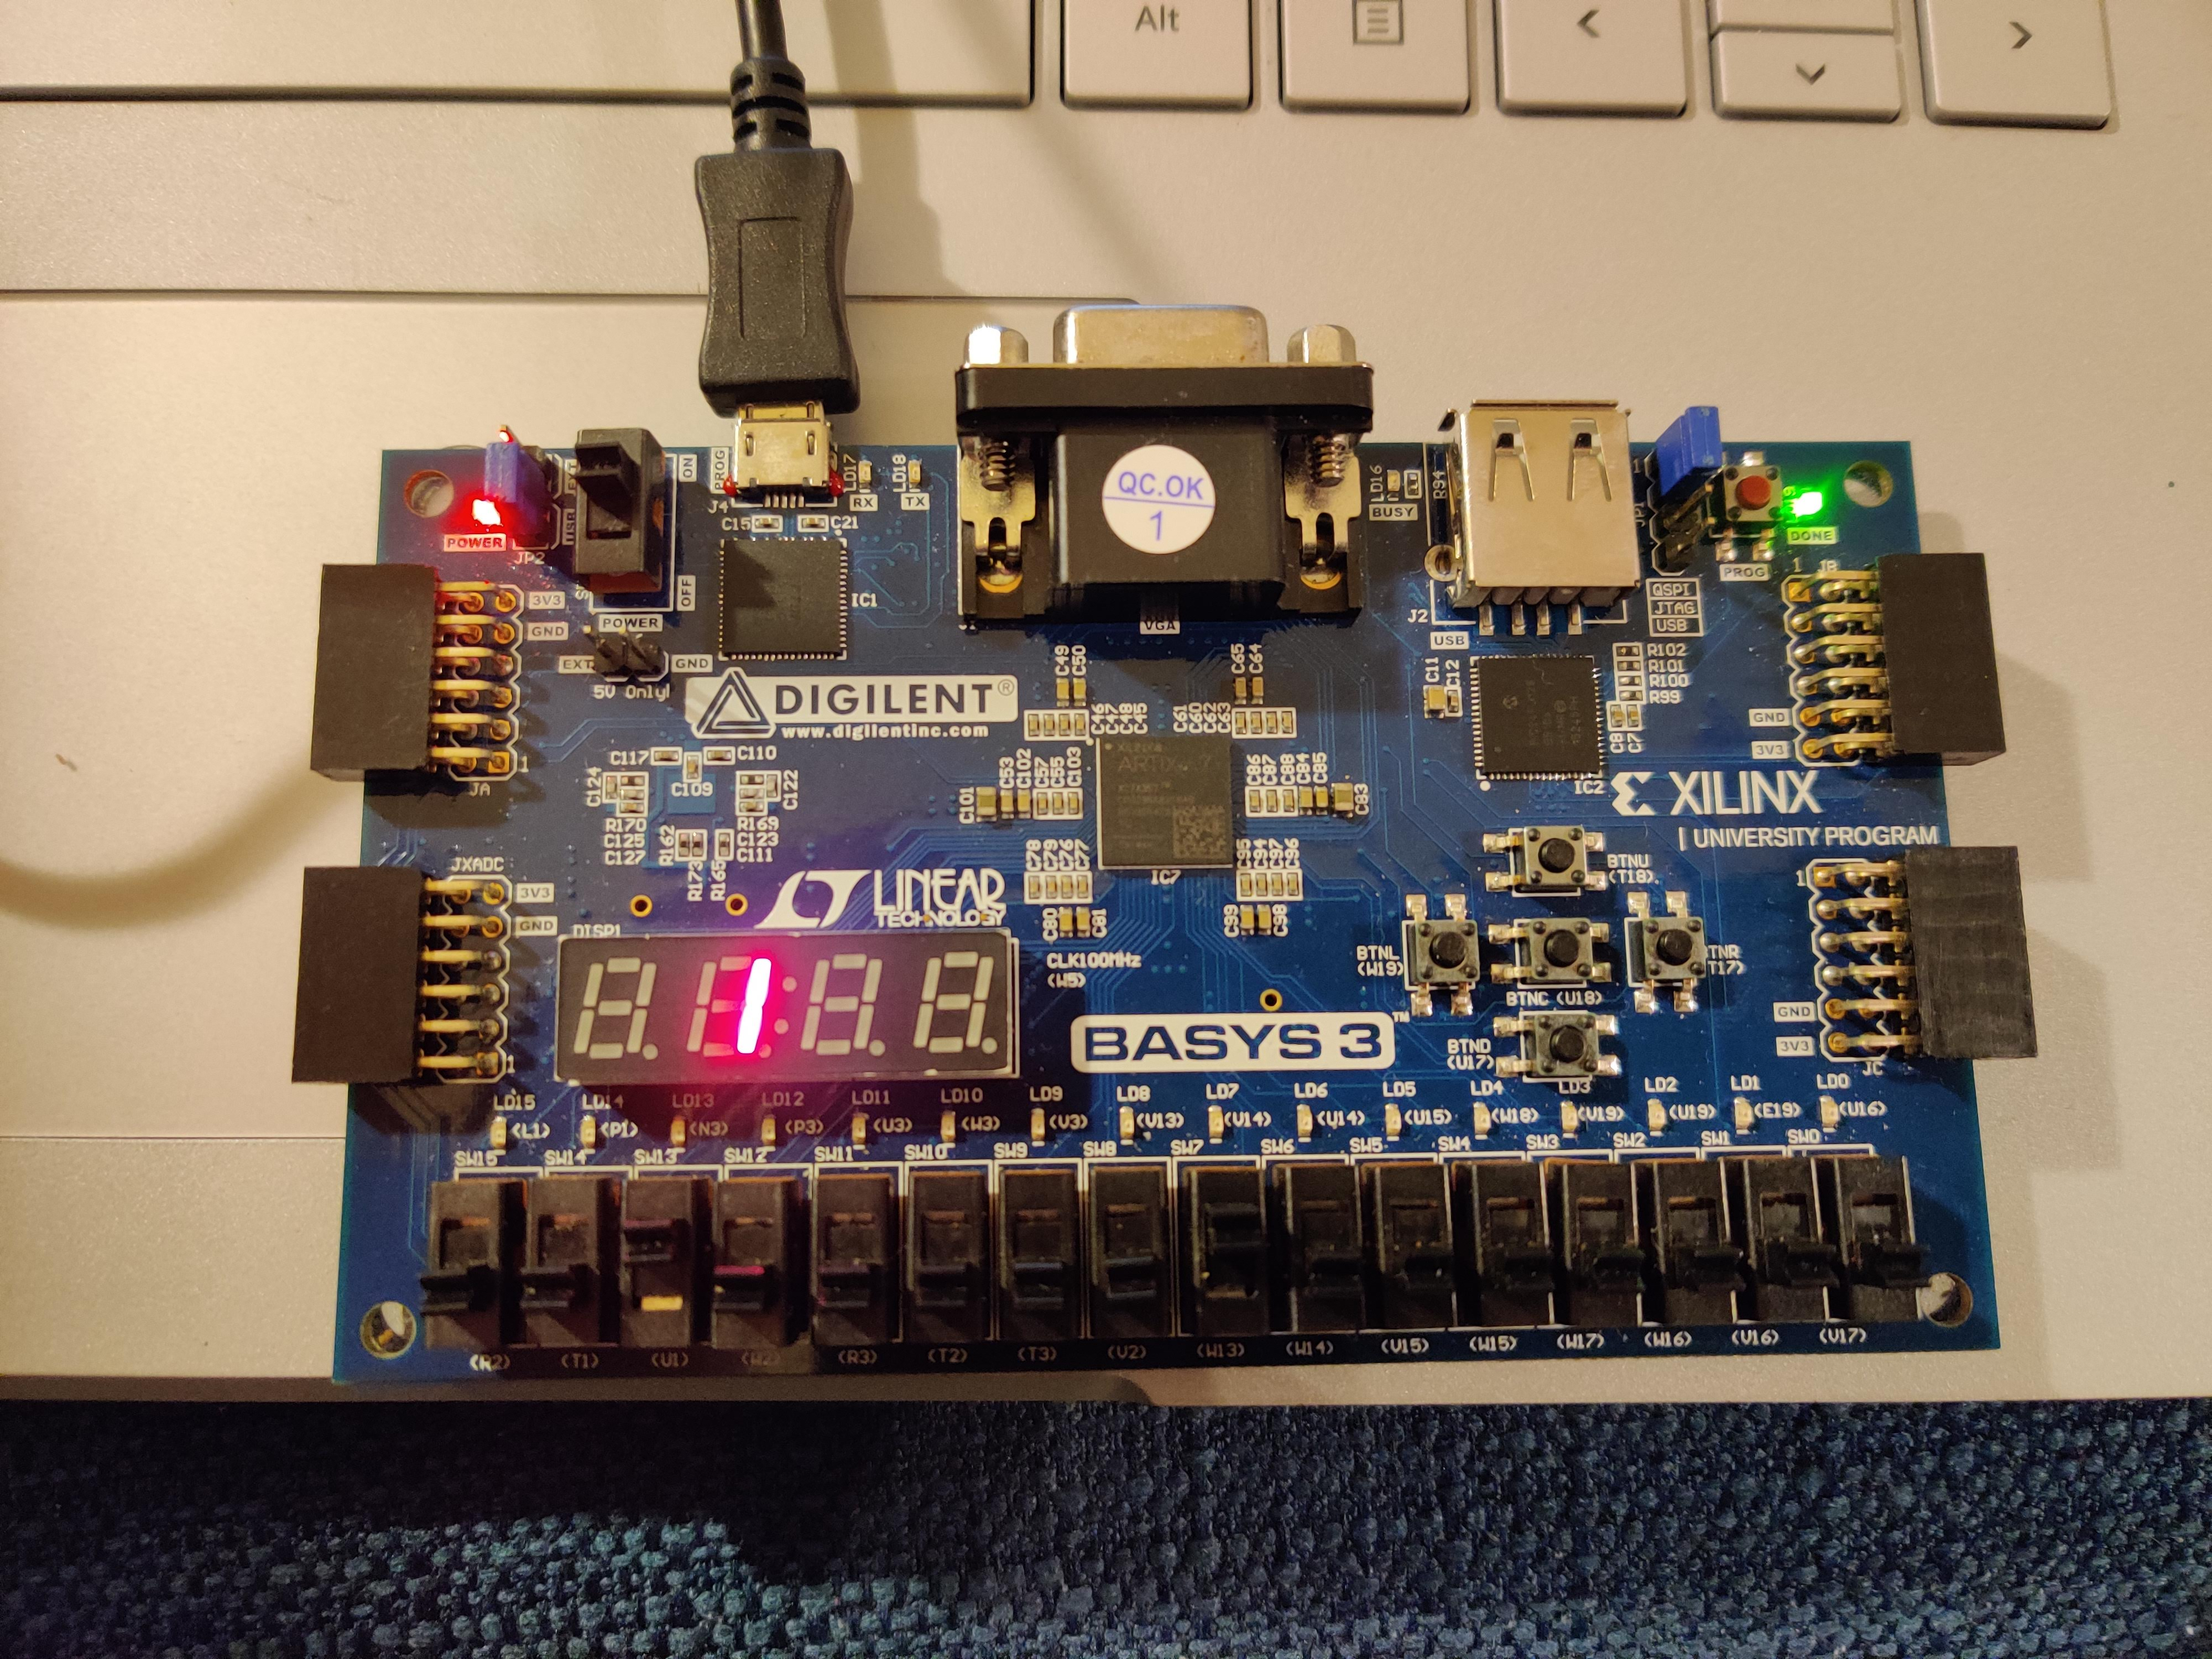
\includegraphics[width=.5\textwidth]{board2}
	\caption{2. sw13:12=10, sw7=1, OUTPUT = 1}
	\label{fig:b3_2}			
\end{figure}

\begin{figure}[ht]\centering
	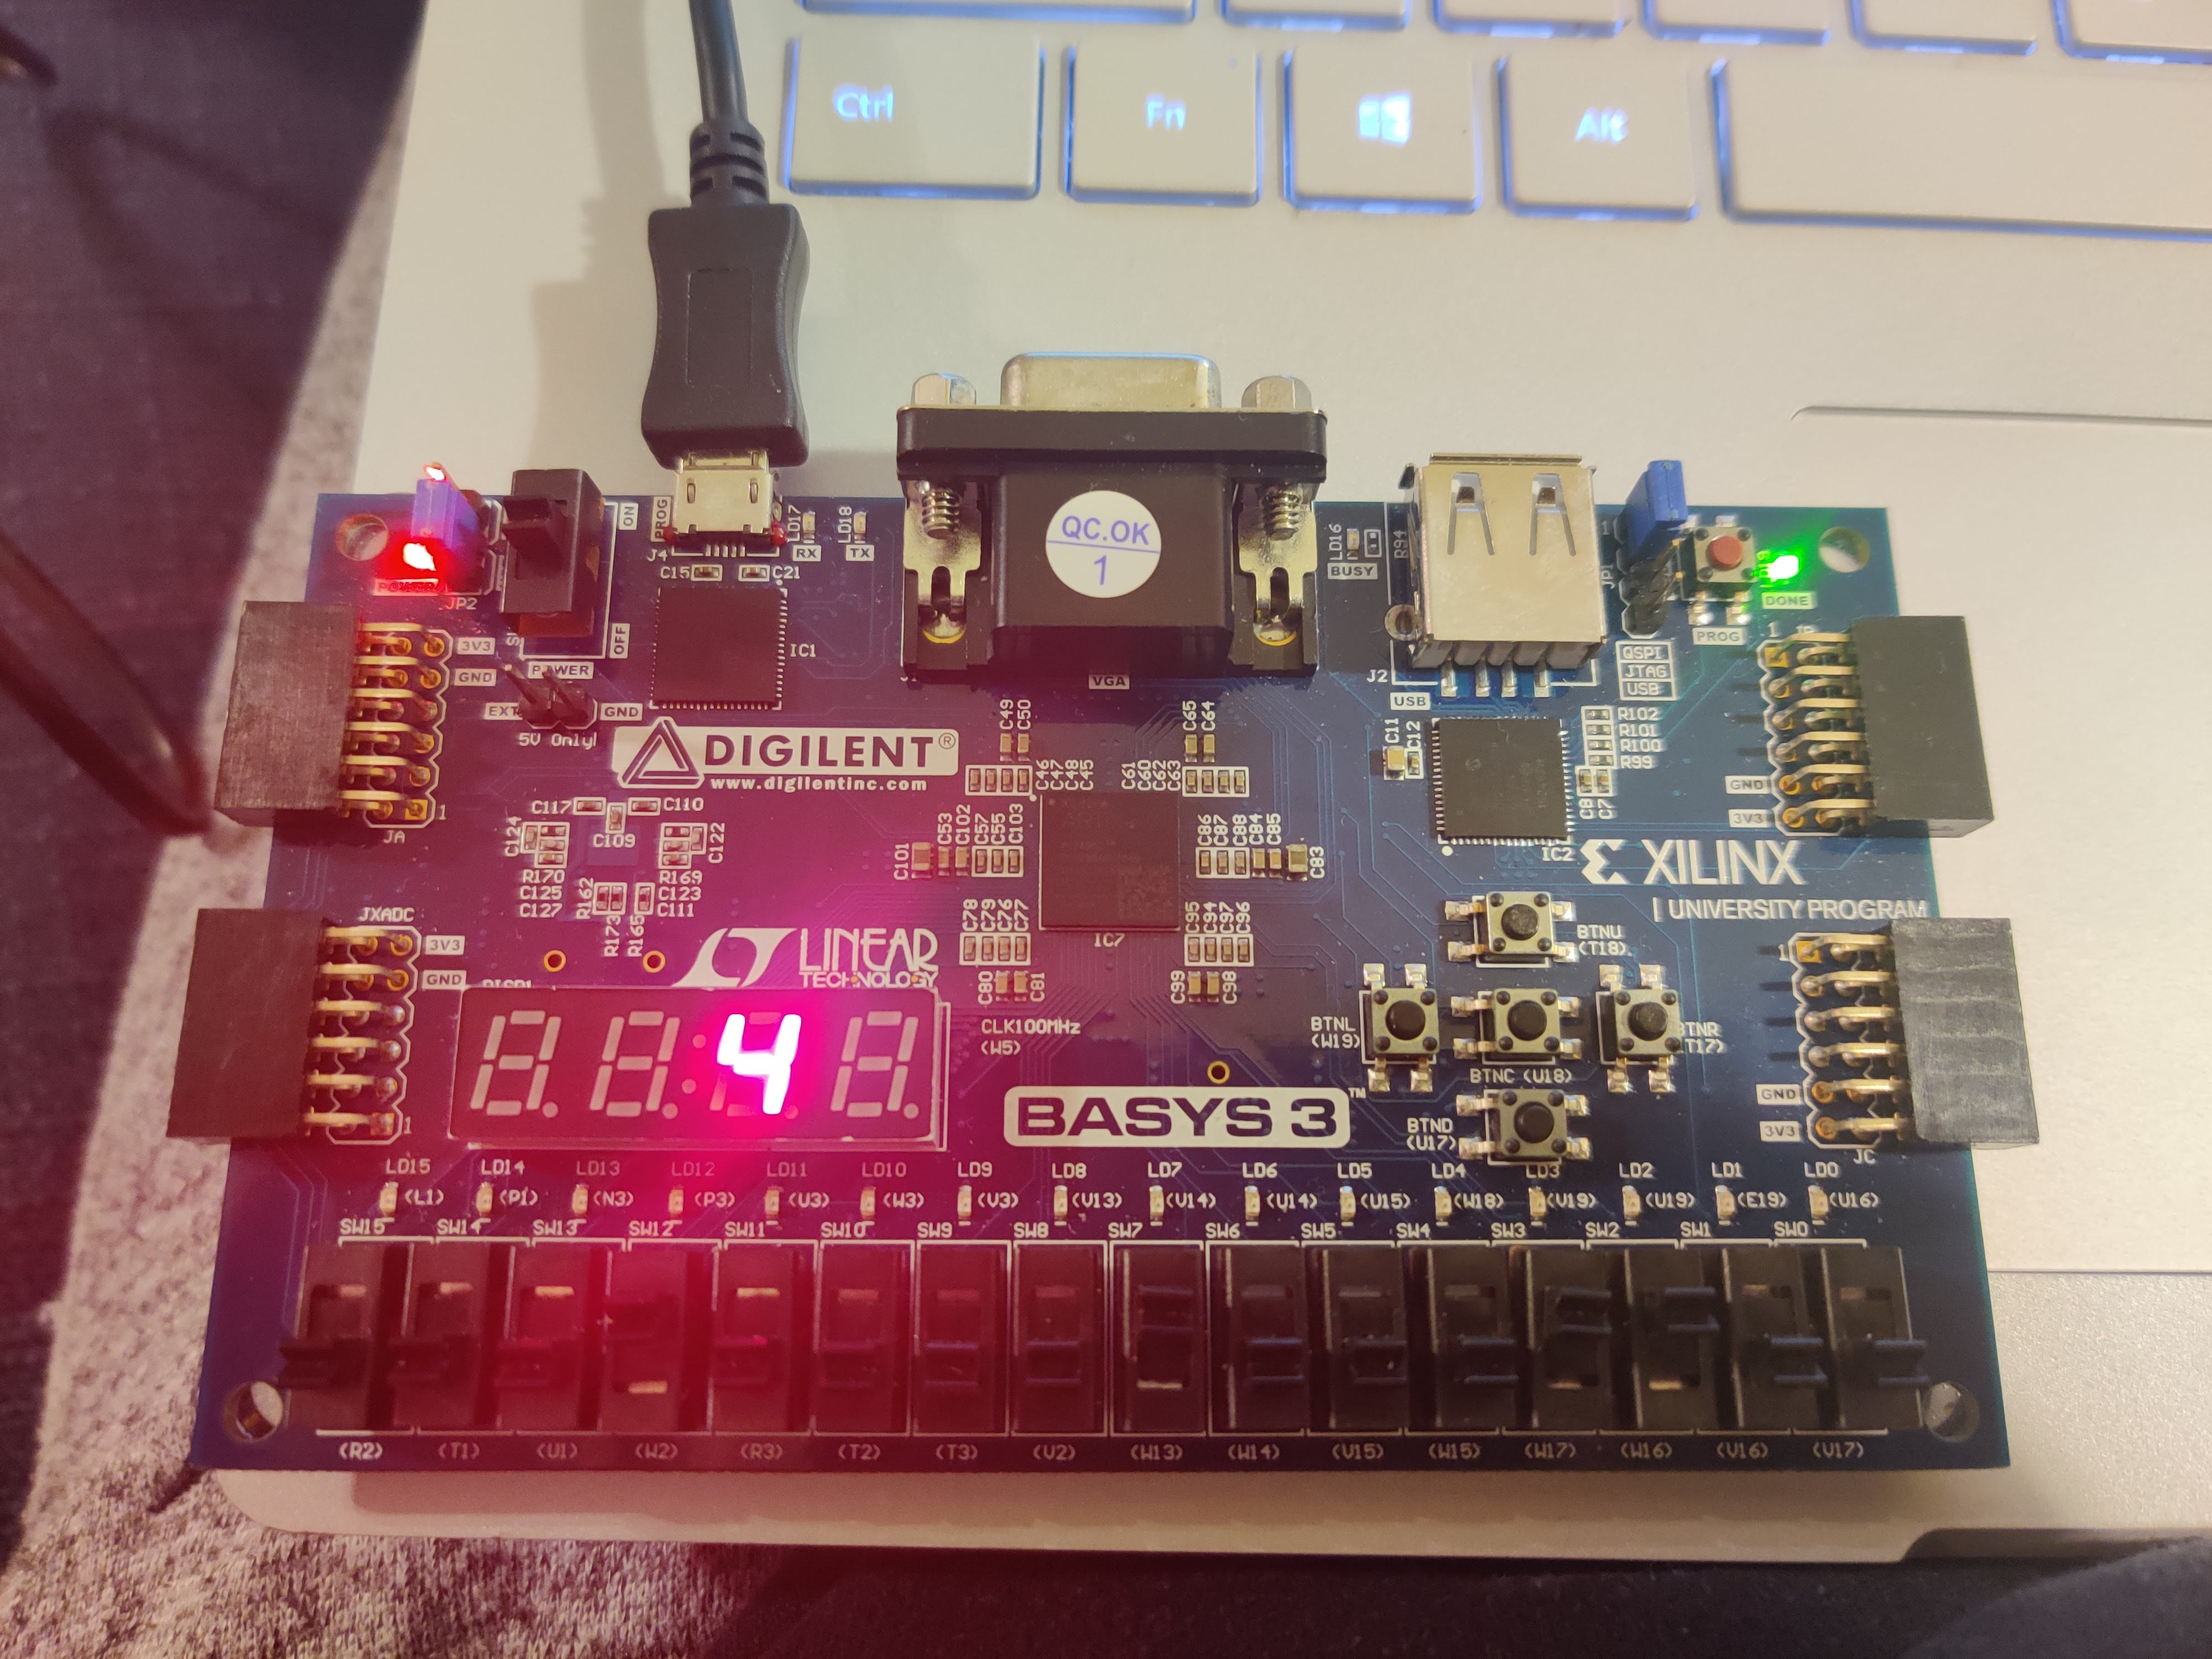
\includegraphics[width=.5\textwidth]{board3}
	\caption{3. sw13:12=01, sw7=1,  sw3:0=1100, OUTPUT = 4}
	\label{fig:b3_3}			
\end{figure}

\begin{figure}[ht]\centering
	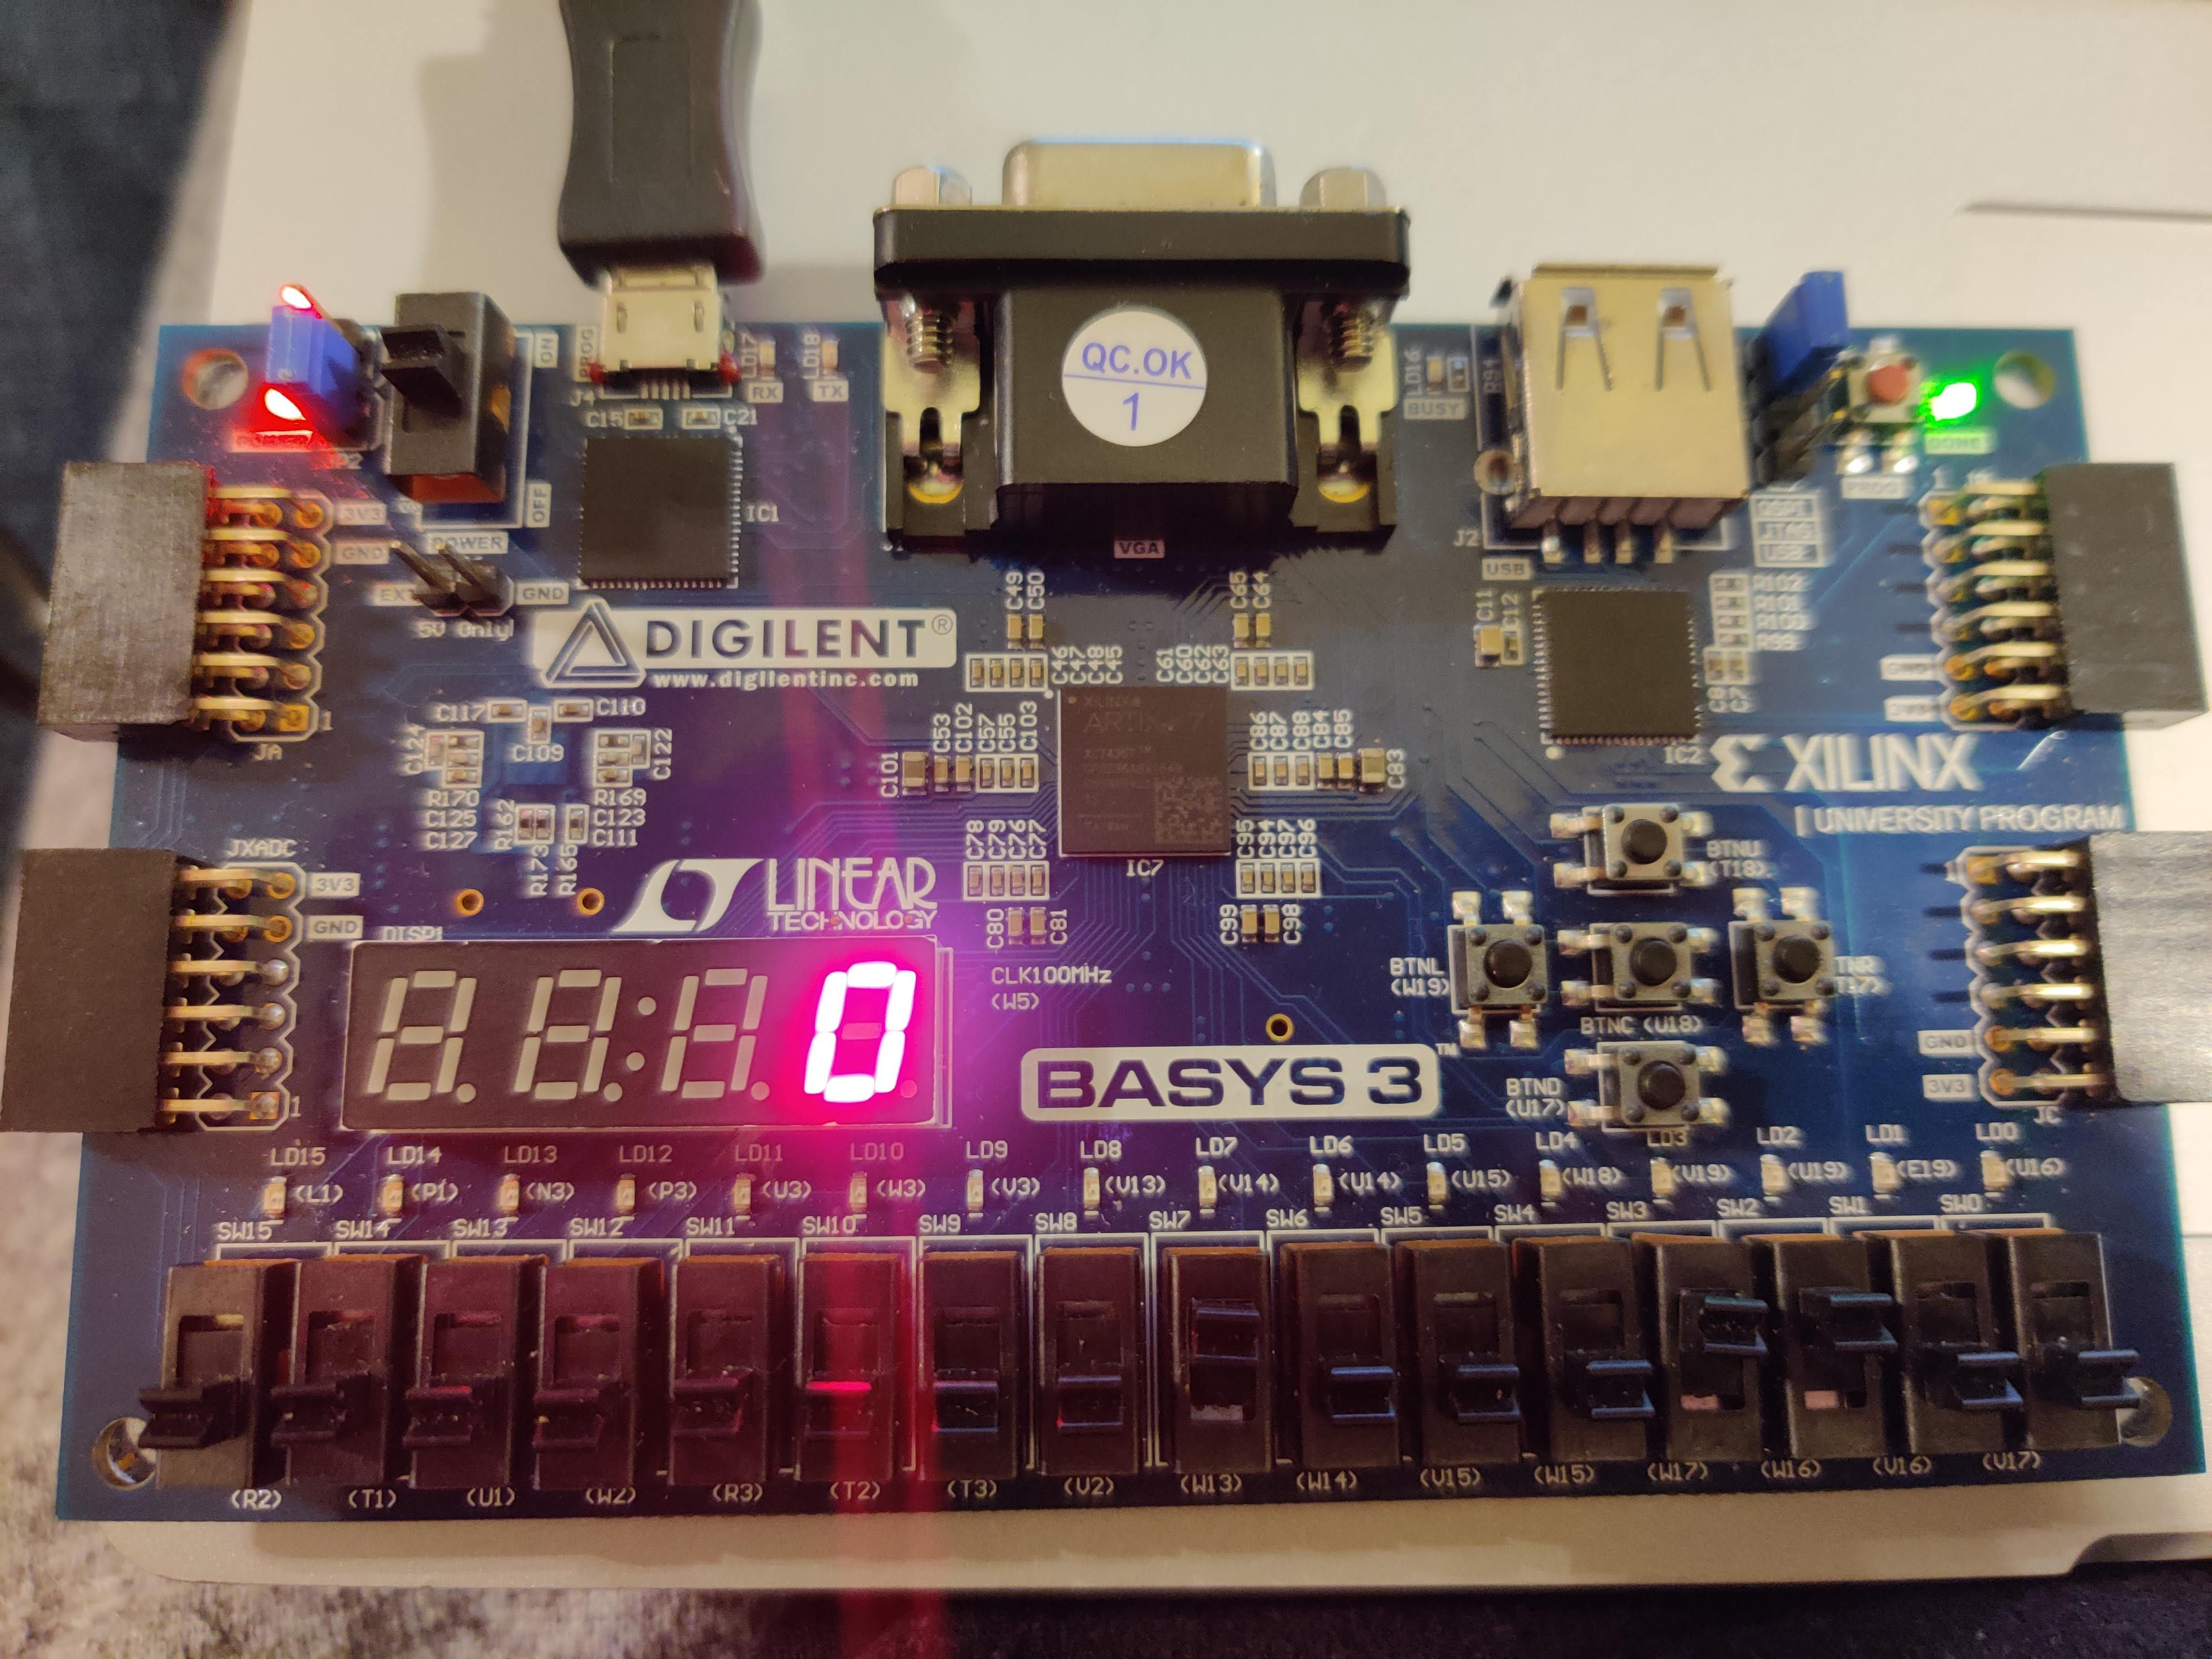
\includegraphics[width=.5\textwidth]{board4}
	\caption{4. sw13:12=00, sw7=1, sw3:0=1100, OUTPUT = 0}
	\label{fig:b3_4}			
\end{figure}

\begin{figure}[ht]\centering
	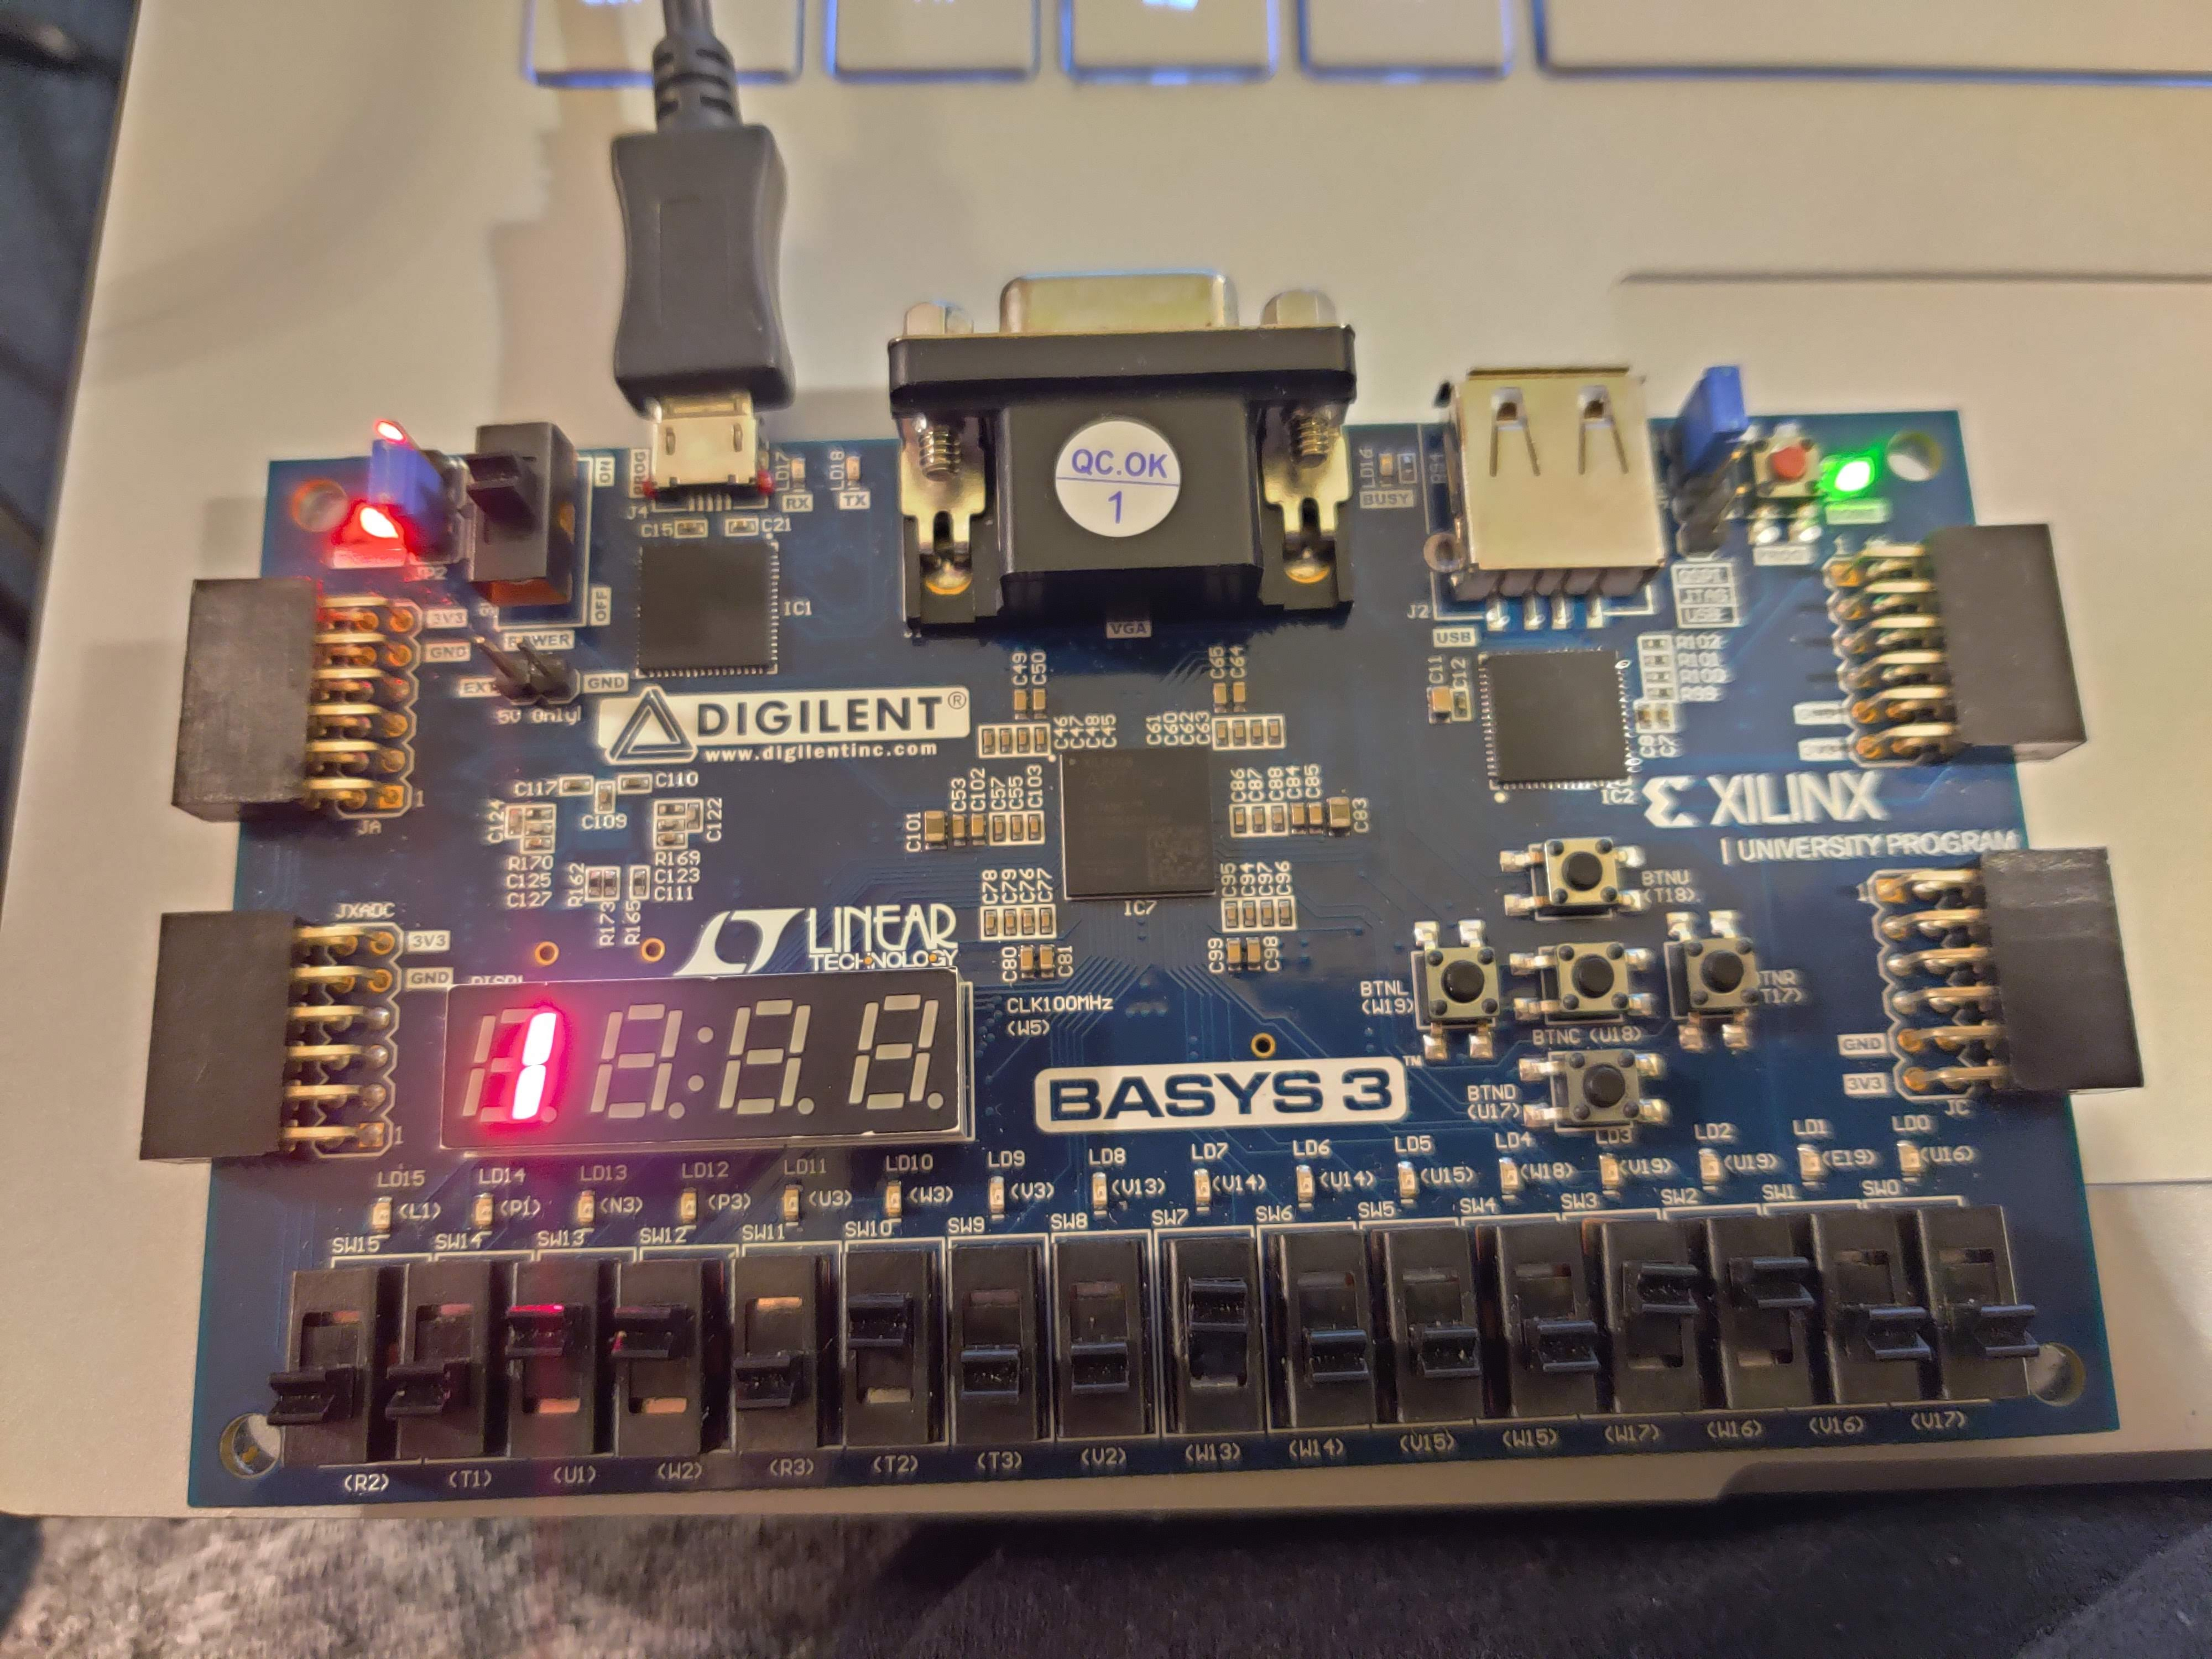
\includegraphics[width=.5\textwidth]{board5}
	\caption{5. sw13:12=11, sw10=1, sw7=1, sw3:0=1100, OUTPUT = 1}
	\label{fig:b3_5}			
\end{figure}

\begin{figure}[ht]\centering
	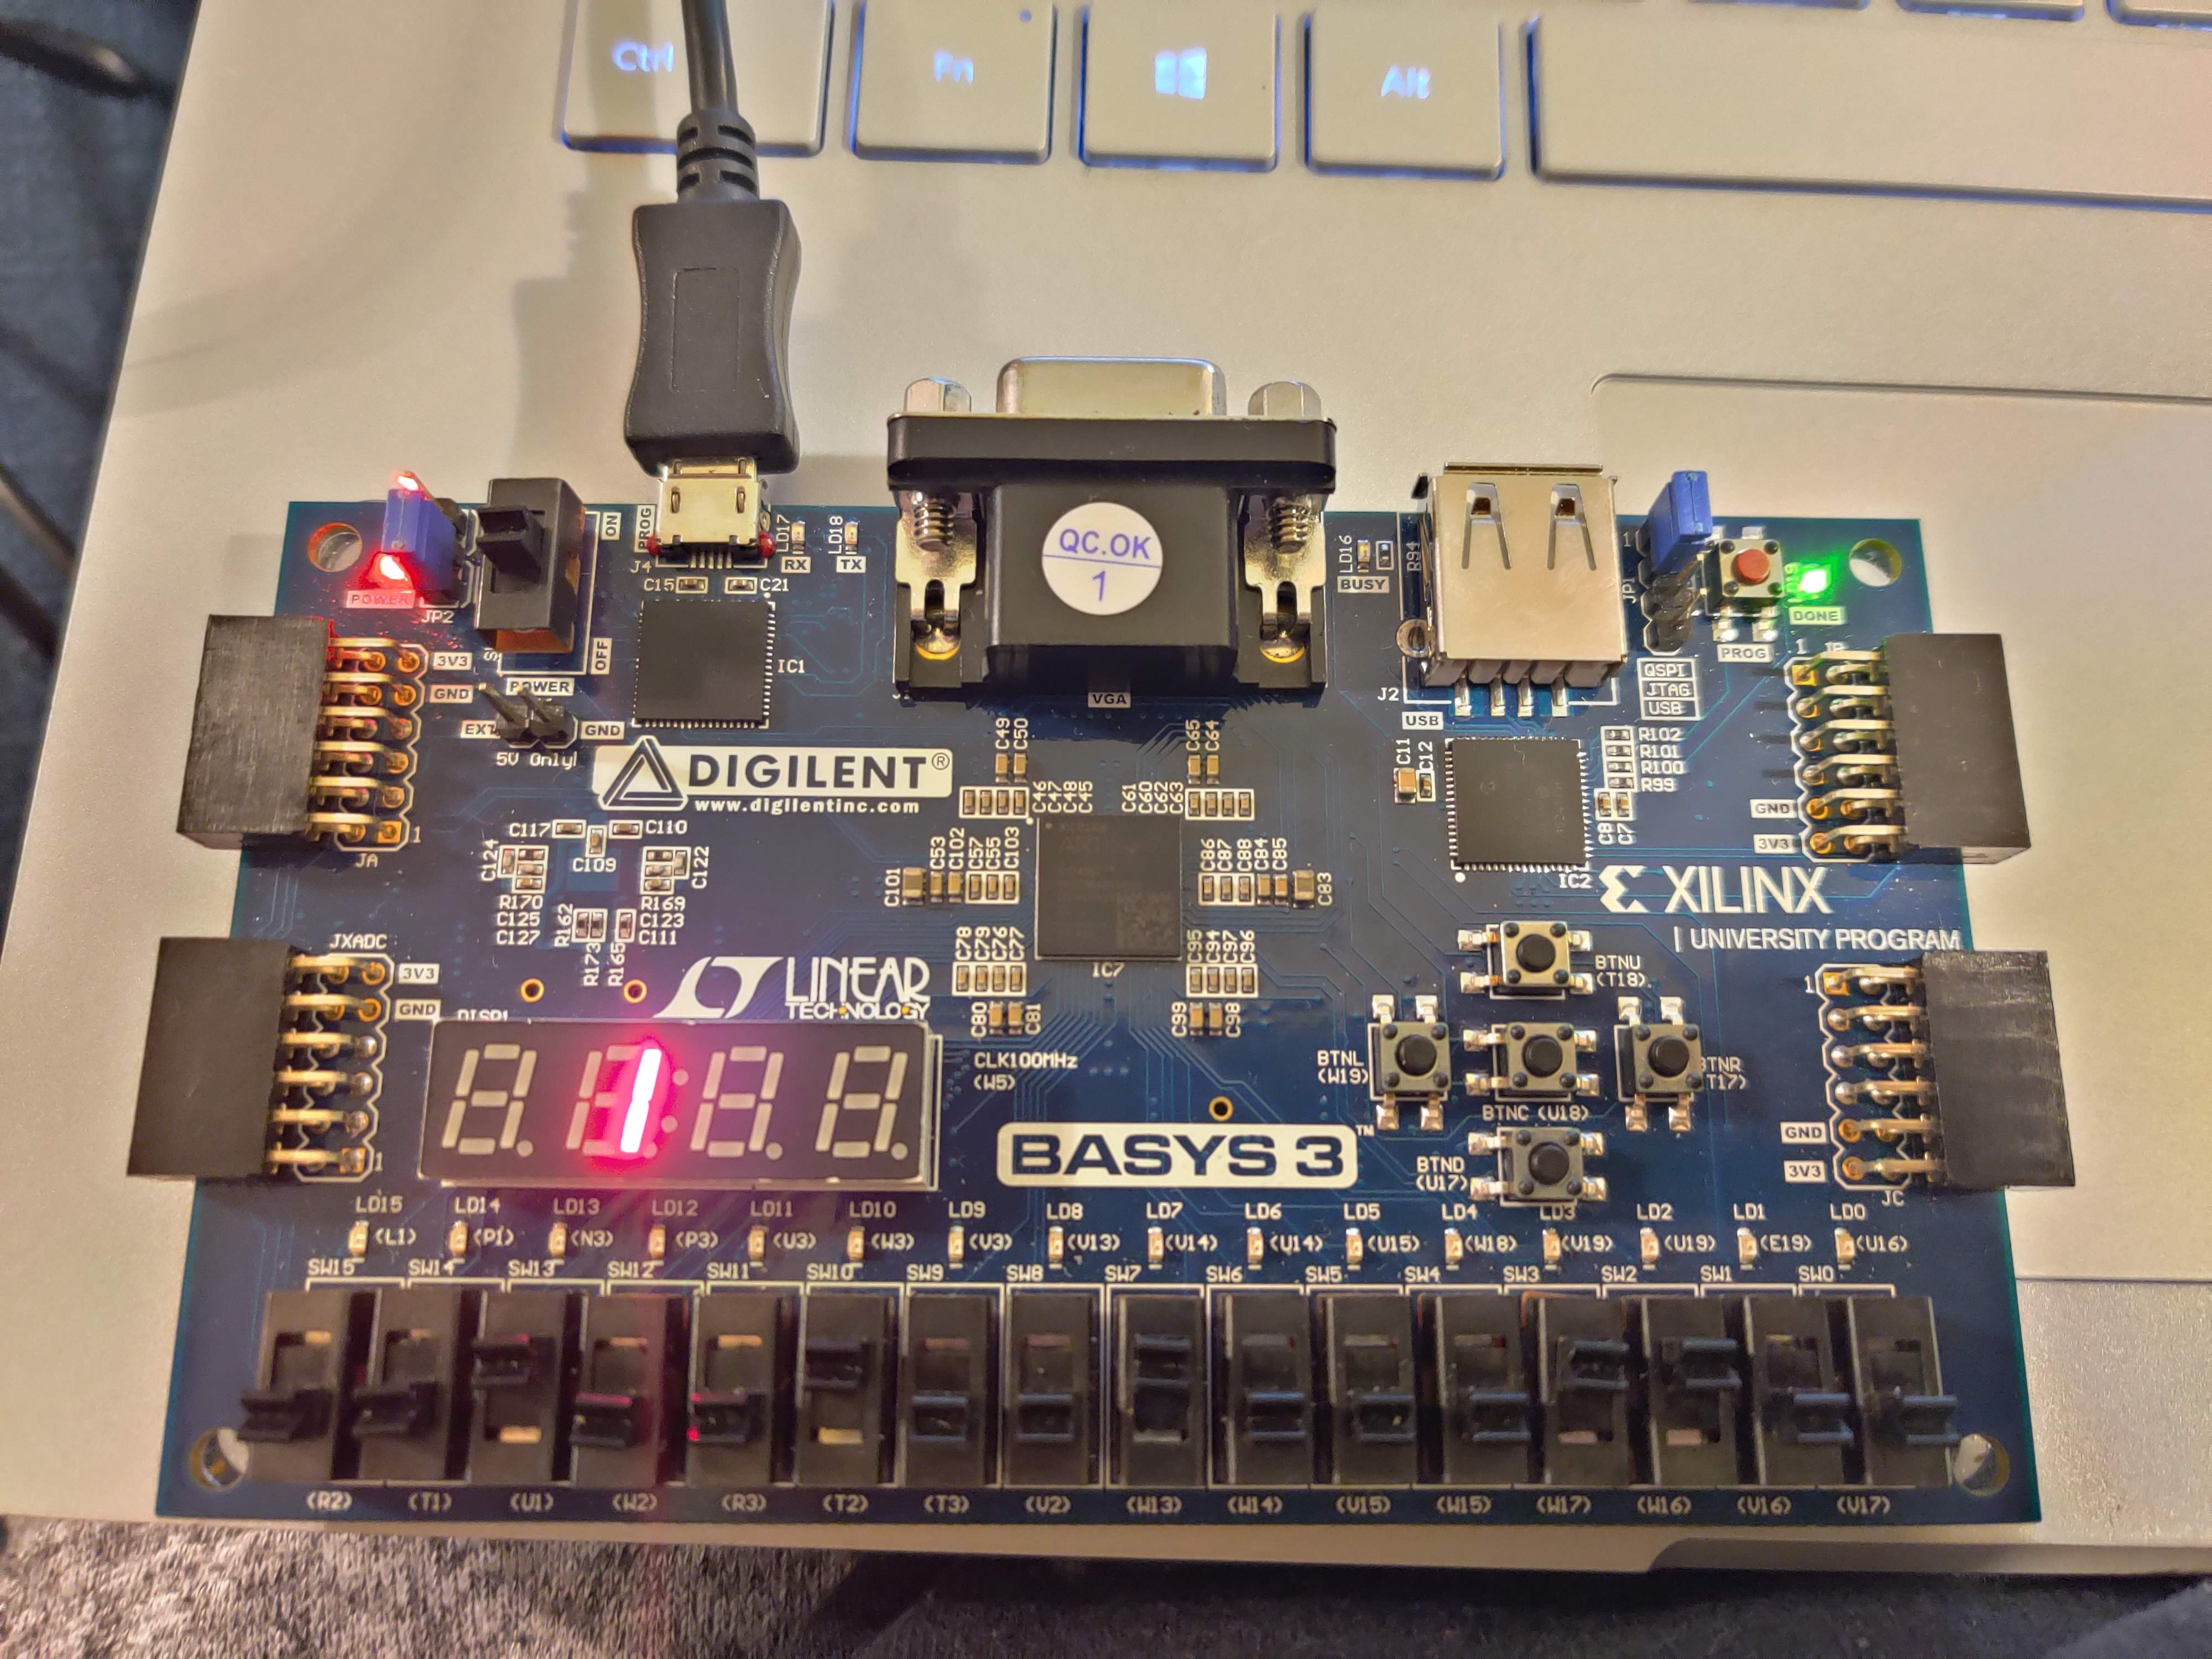
\includegraphics[width=.5\textwidth]{board6}
	\caption{6. sw13:12=10, sw10=1, sw7=1, sw3:0=1100, OUTPUT = 1}
	\label{fig:b3_6}			
\end{figure}

\begin{figure}[ht]\centering
	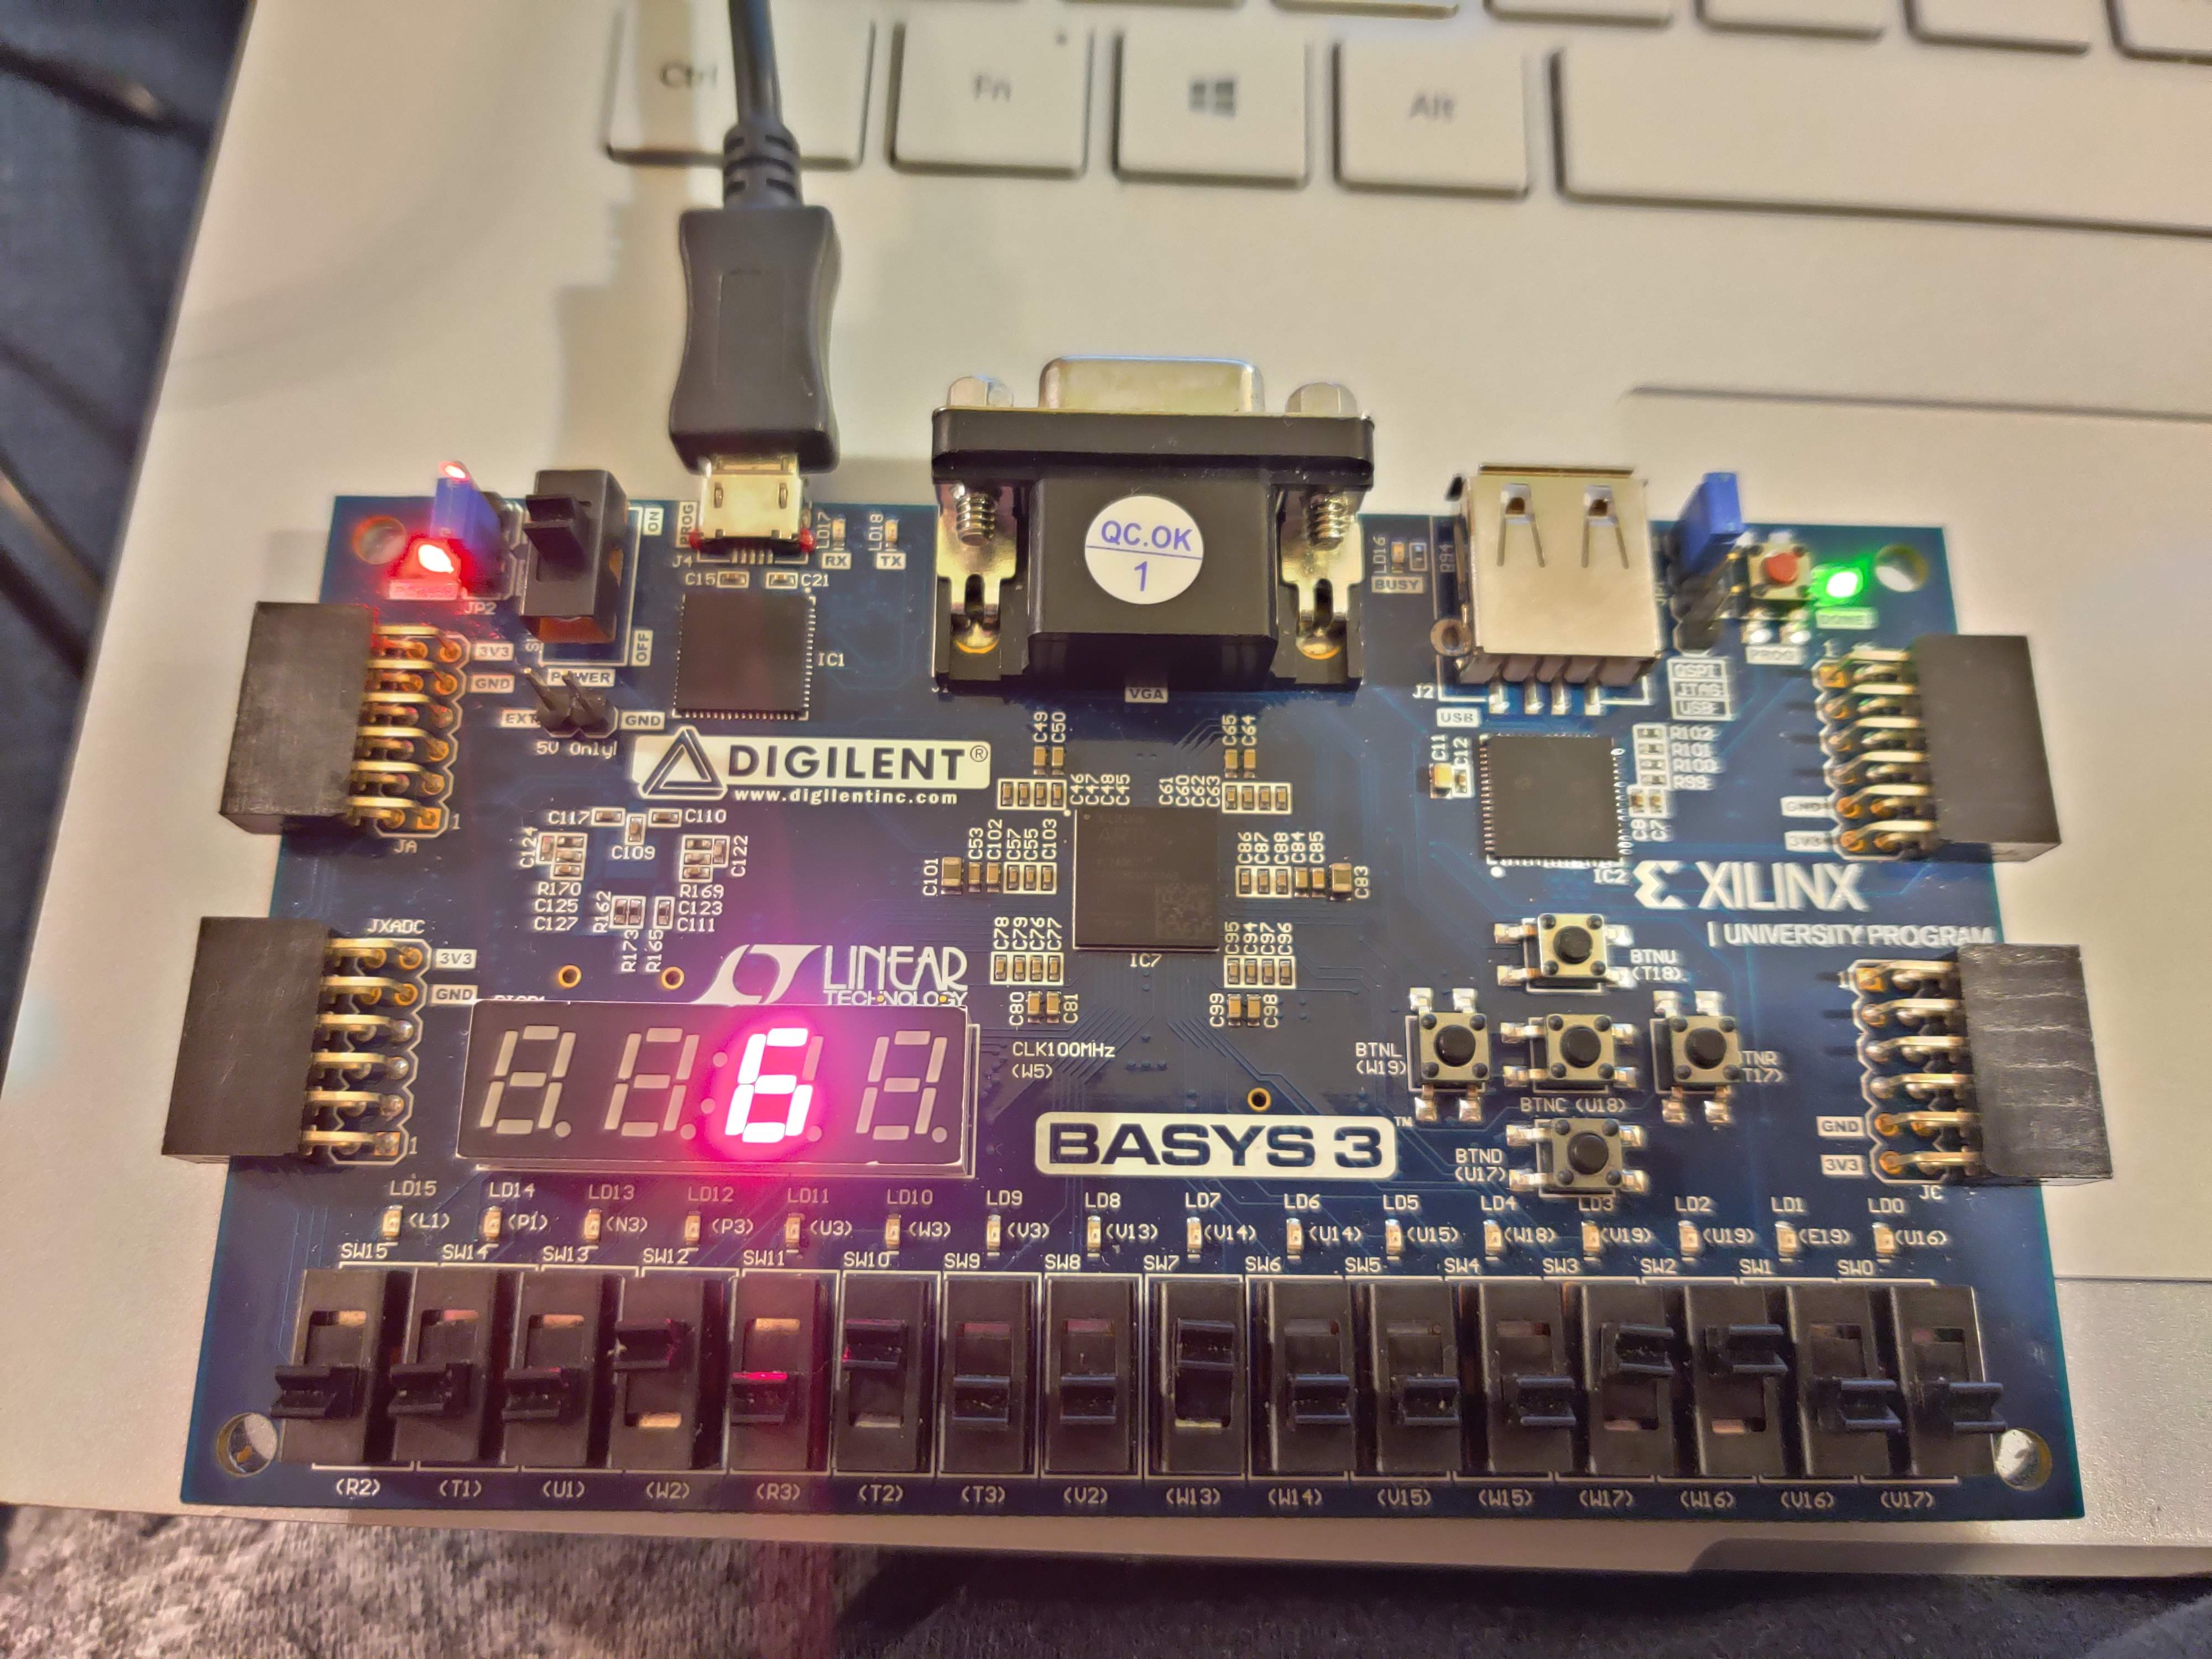
\includegraphics[width=.5\textwidth]{board7}
	\caption{7. sw13:12=01, sw10=1, sw7=1, sw3:0=1100, OUTPUT = 6}
	\label{fig:b3_7}			
\end{figure}

\begin{figure}[ht]\centering
	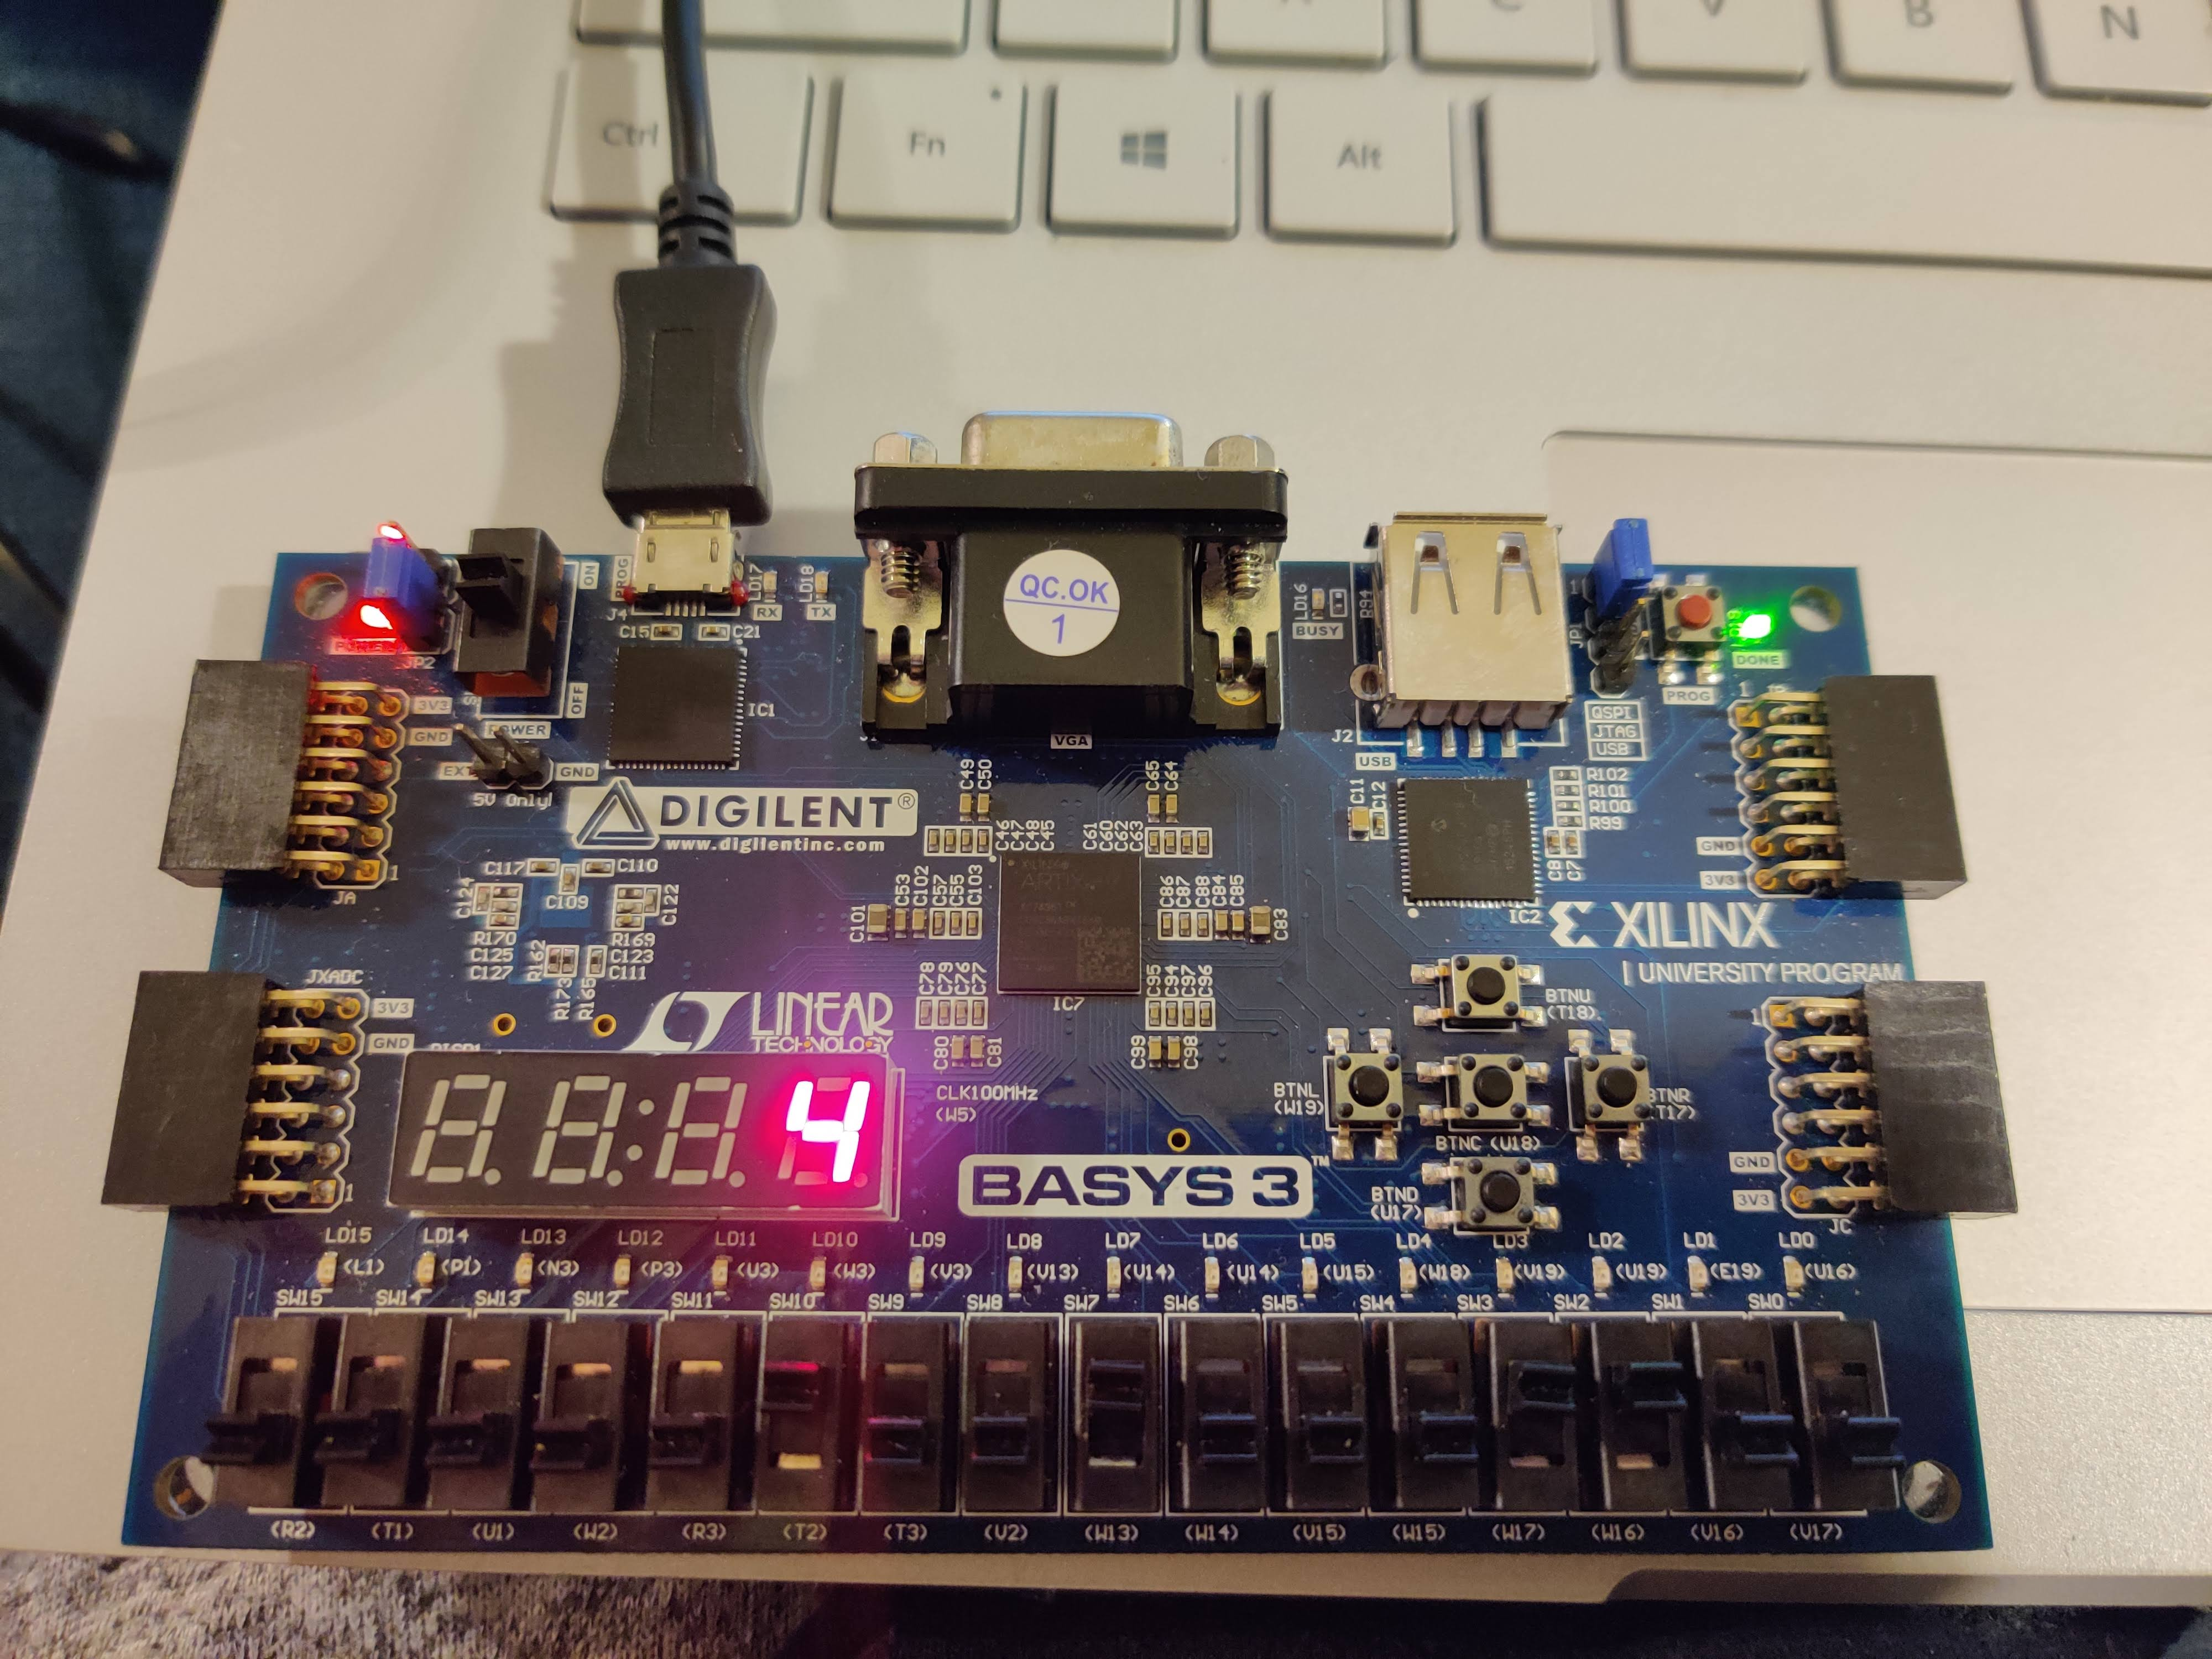
\includegraphics[width=.5\textwidth]{board8}
	\caption{8. sw13:12=00, sw10=1, sw7=1, sw3:0=1100, OUTPUT = 4}
	\label{fig:b3_8}			
\end{figure}

\begin{figure}[ht]\centering
	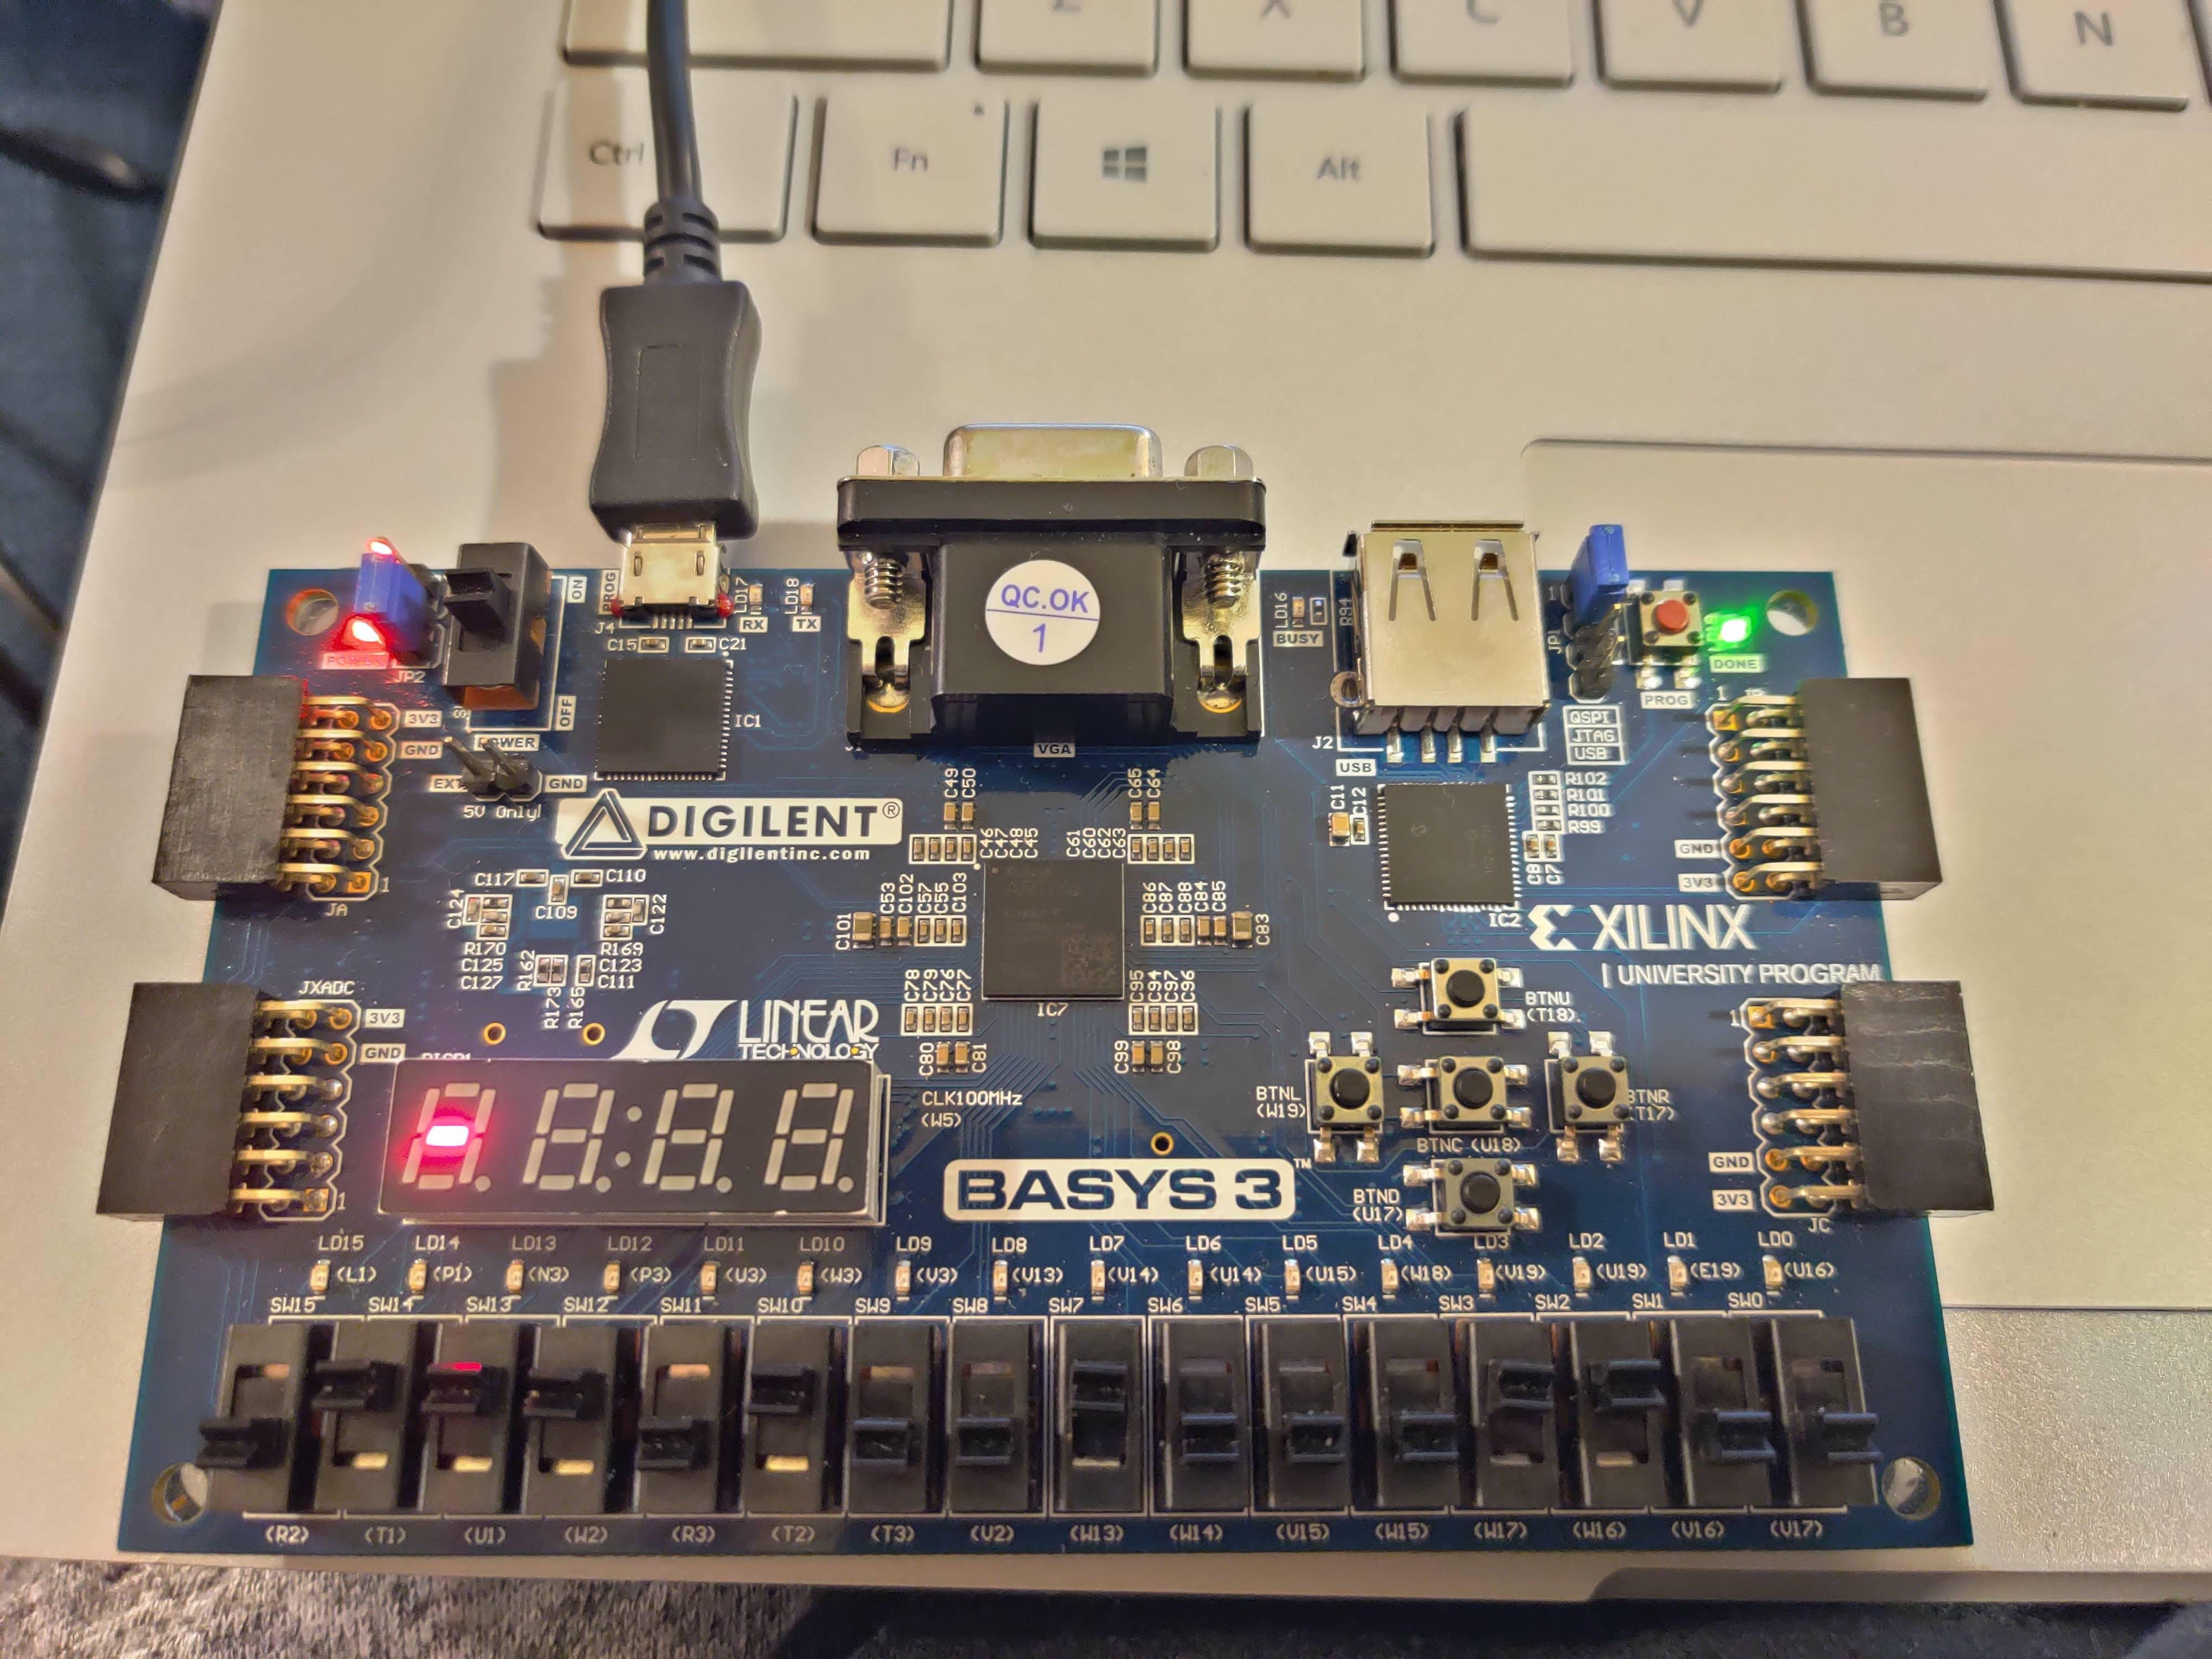
\includegraphics[width=.5\textwidth]{board9}
	\caption{9. sw14=1, sw13:12=11, sw10=1, sw7=1, sw3:0=1100, OUTPUT = -}
	\label{fig:b3_9}			
\end{figure}

\begin{figure}[ht]\centering
	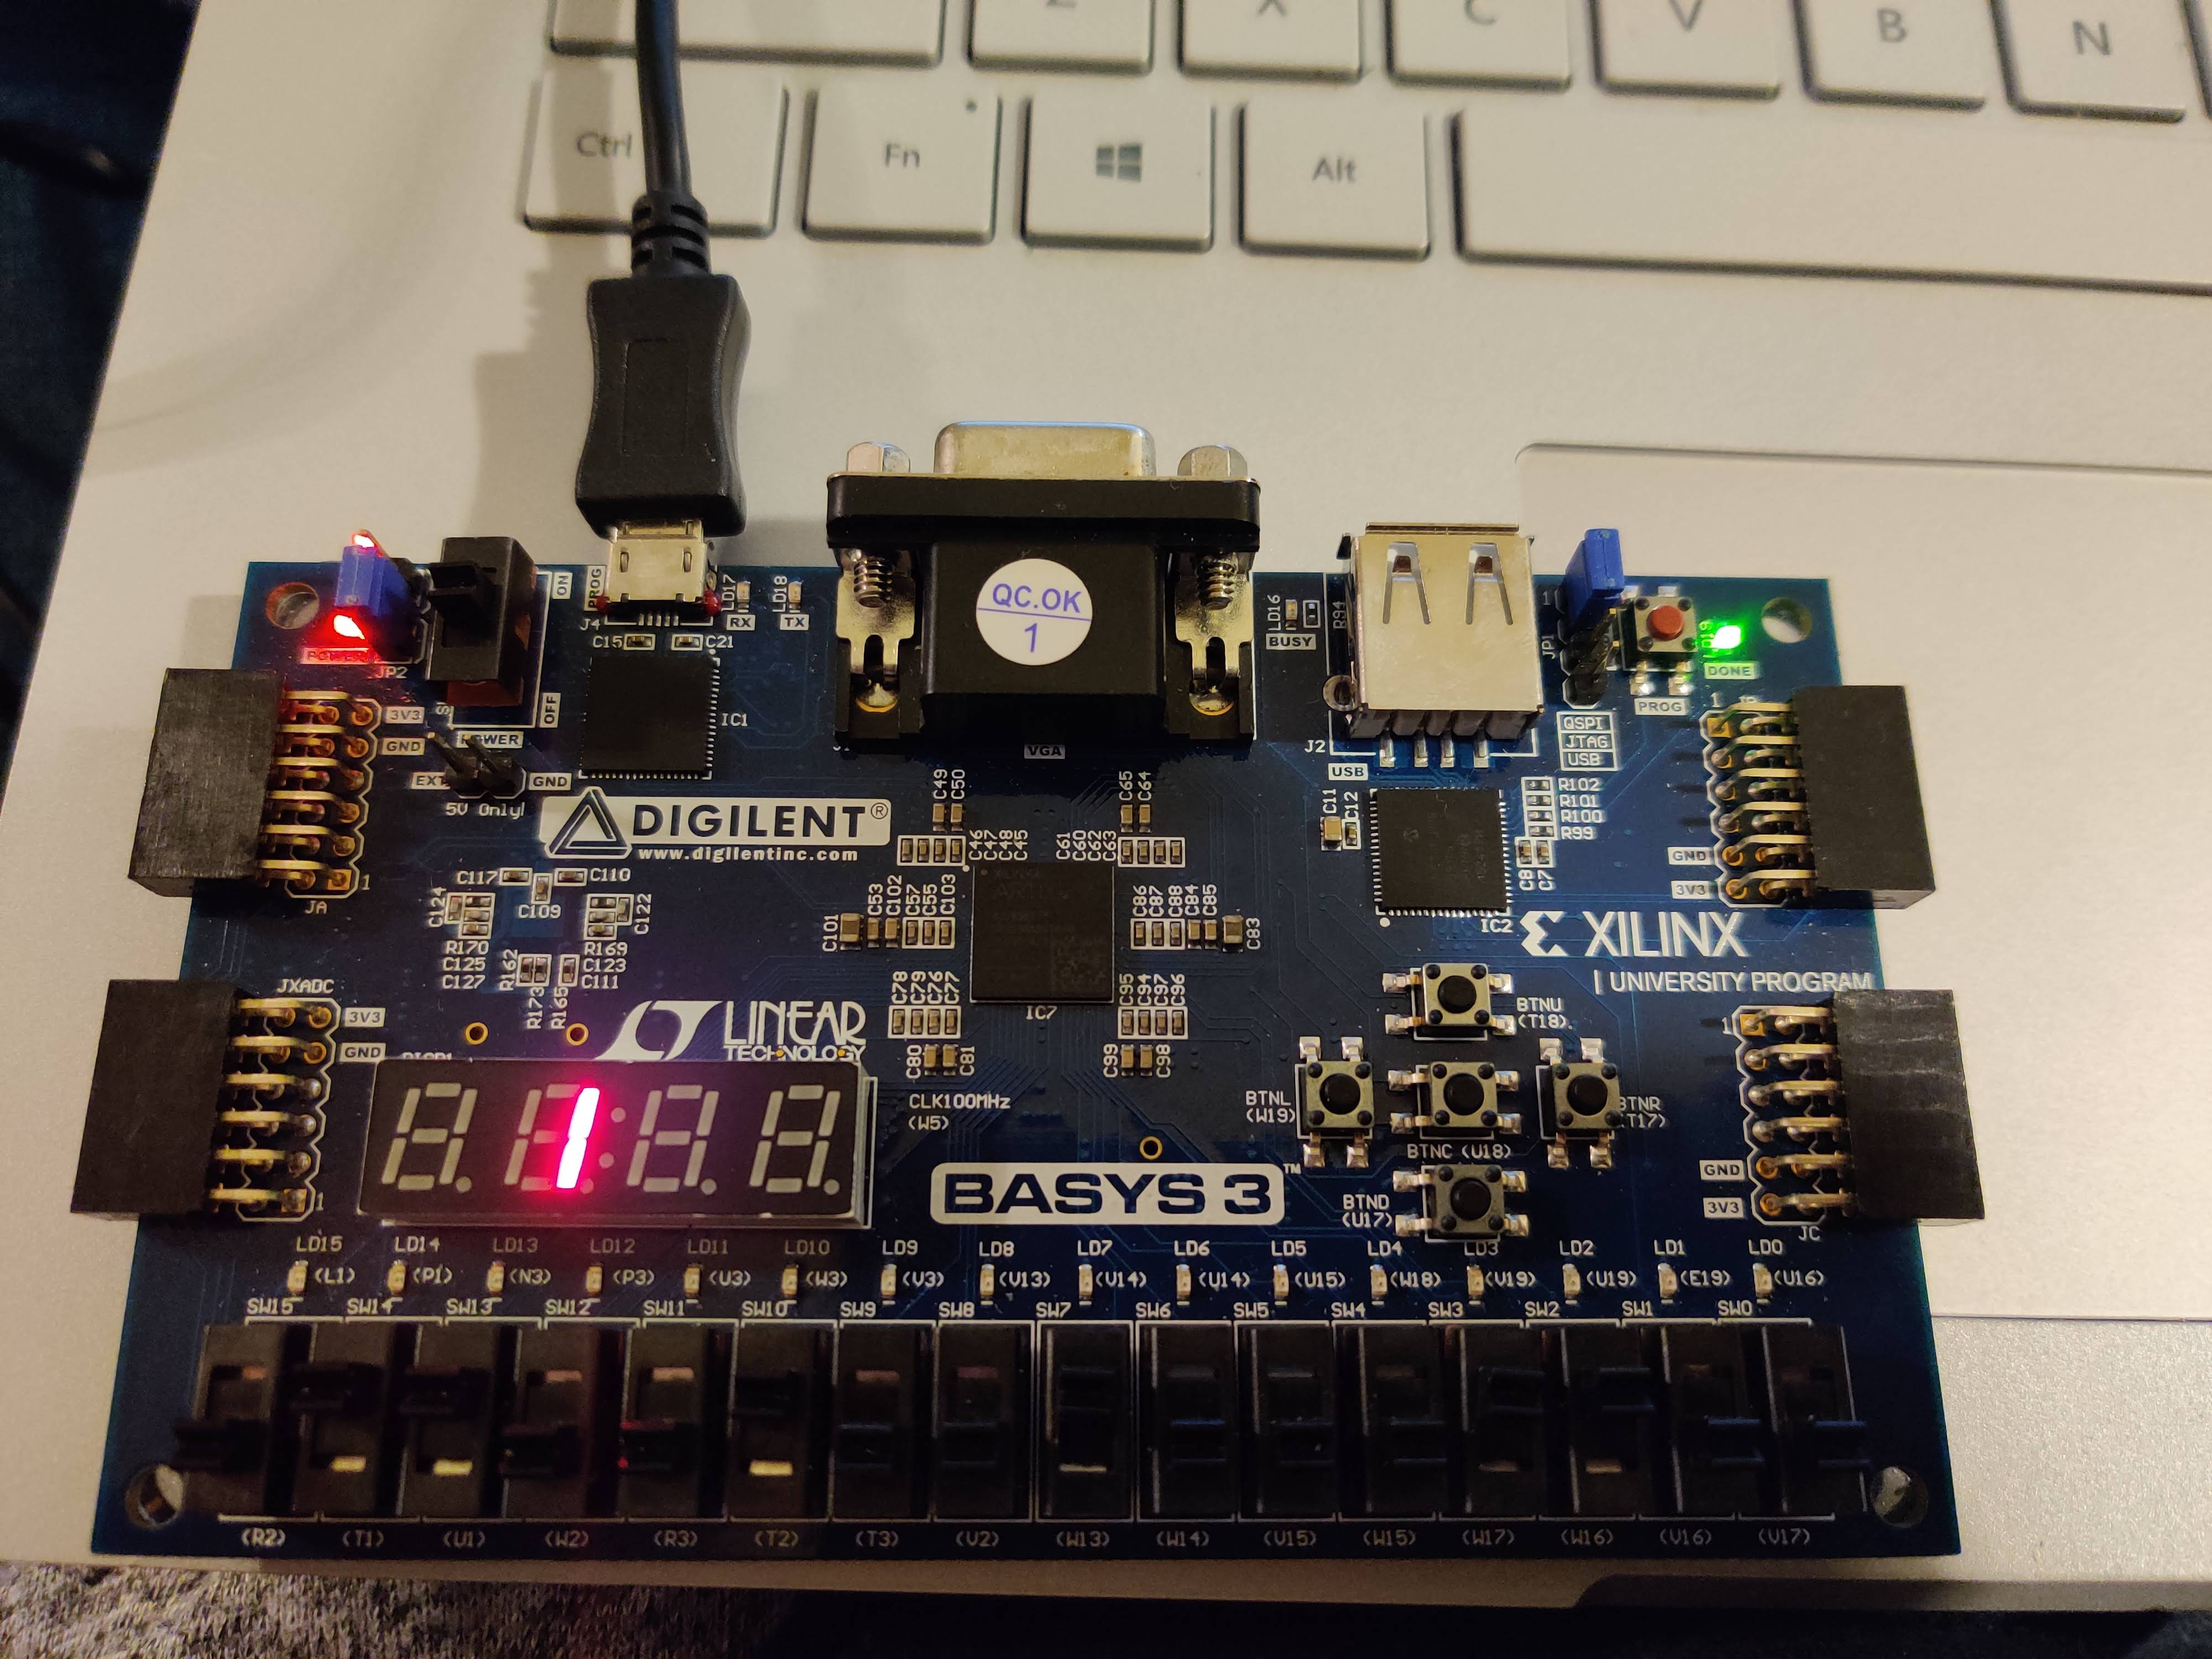
\includegraphics[width=.5\textwidth]{board10}
	\caption{10. sw14=1 sw13:12=10, sw10=1, sw7=1, sw3:0=1100, OUTPUT = 1}
	\label{fig:b3_10}			
\end{figure}

\begin{figure}[ht]\centering
	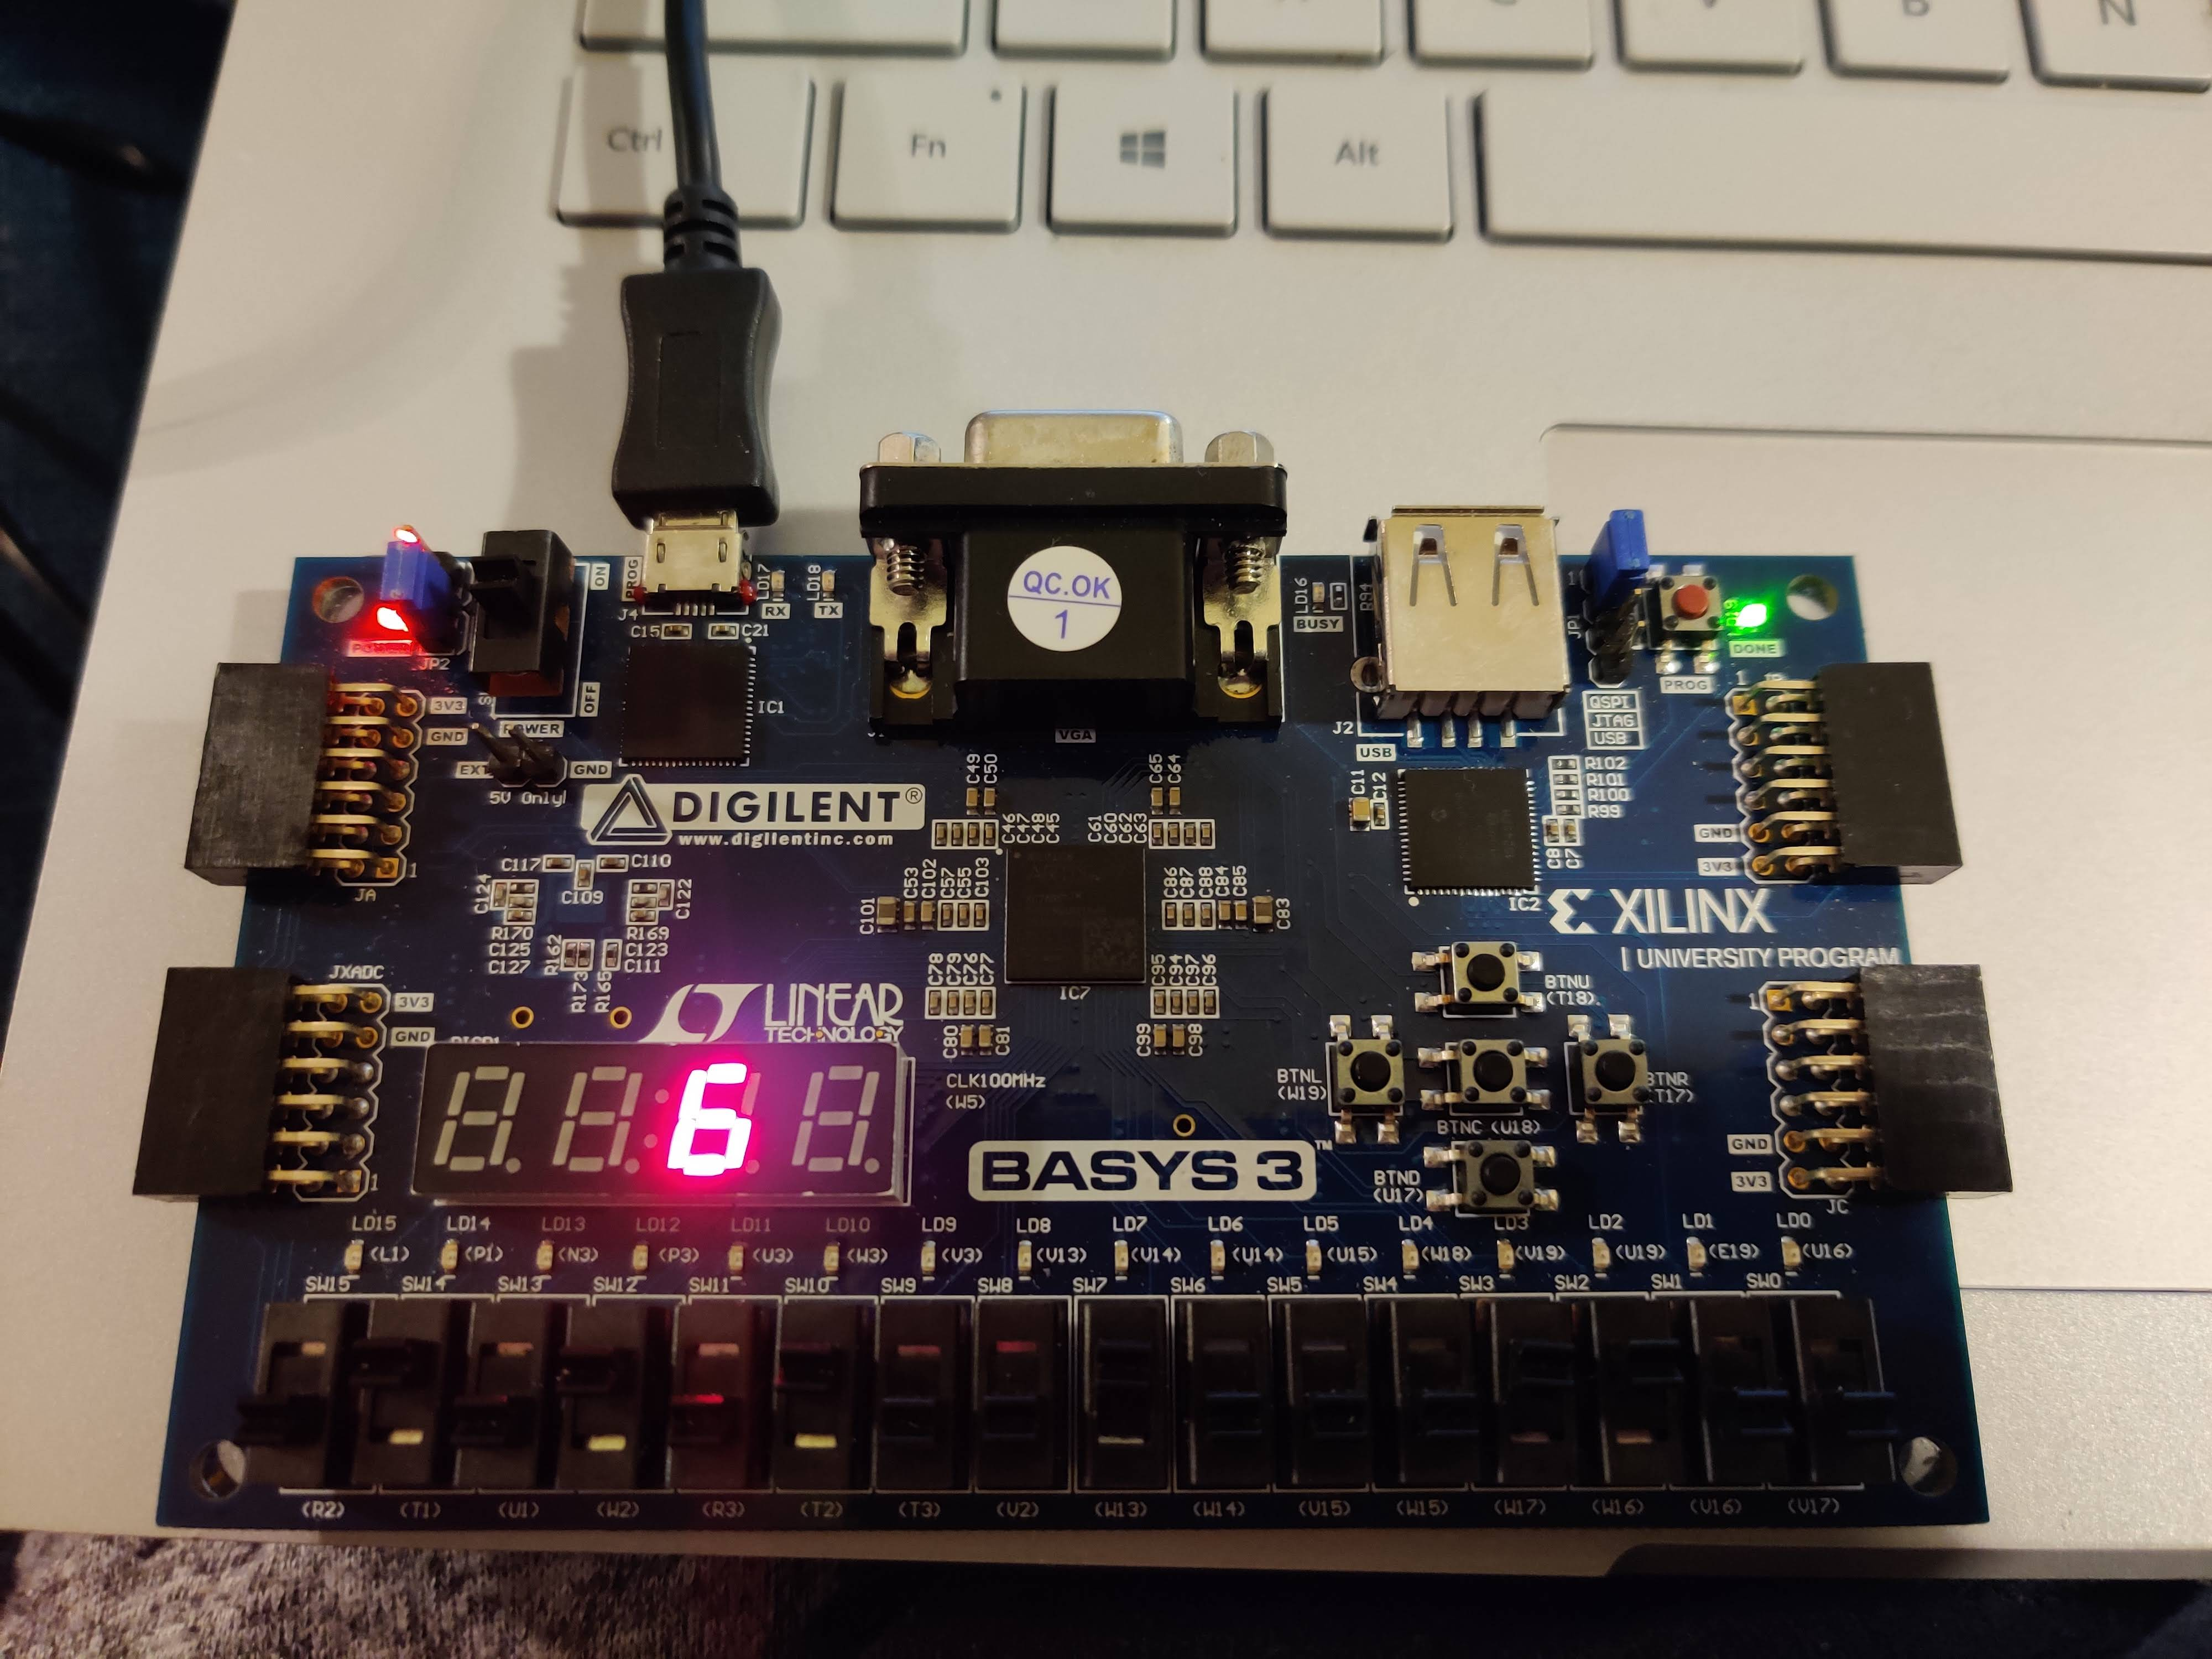
\includegraphics[width=.5\textwidth]{board11}
	\caption{11. sw14=1 sw13:12=01, sw10=1, sw7=1, sw3:0=1100, OUTPUT = 6}
	\label{fig:b3_11}			
\end{figure}

\begin{figure}[ht]\centering
	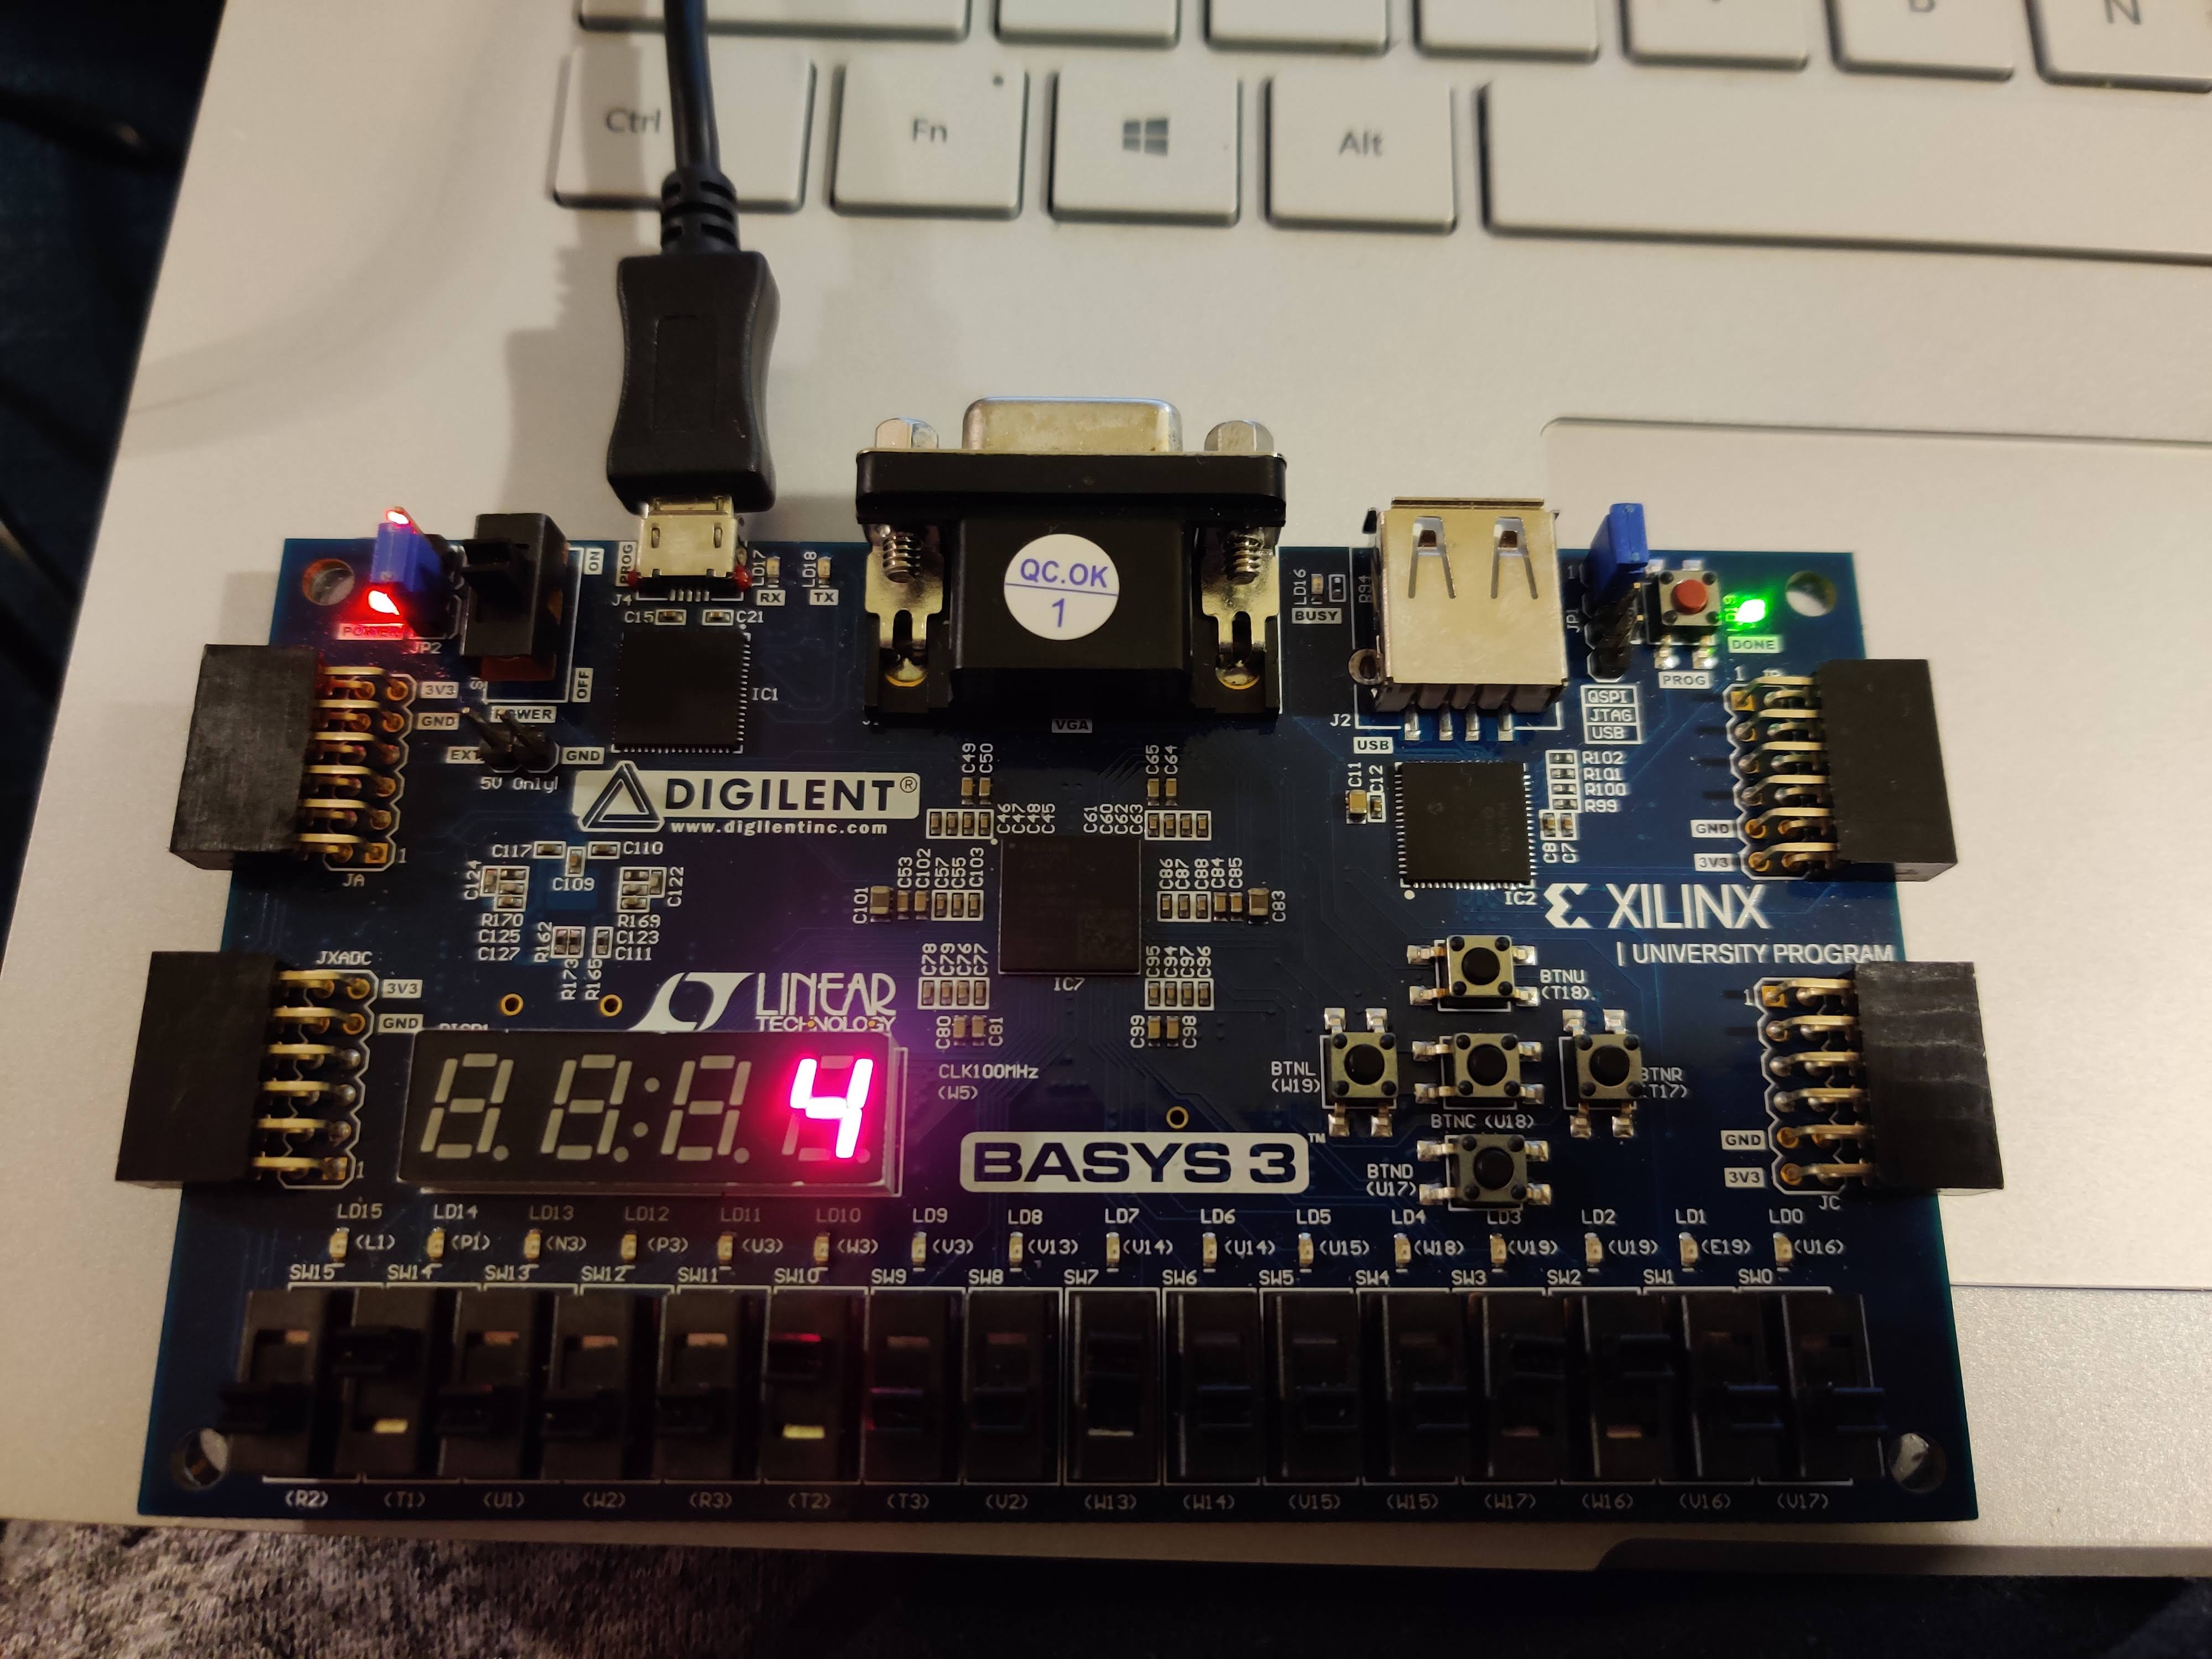
\includegraphics[width=.5\textwidth]{board12}
	\caption{12. sw14=1 sw13:12=00, sw10=1, sw7=1, sw3:0=1100, OUTPUT = 4}
	\label{fig:b3_12}			
\end{figure}

\end{document}
